\section{Methodology}



We employed the publicly available \textbf{Sleep-EDF} dataset for automated sleep stage classification. This dataset consists of two primary file types: Polysomnographic (PSG) recordings in European Data Format (EDF) and corresponding Hypnogram annotation files. The EDF files contain multi-channel biosignals, including EEG, while the Hypnogram files provide ground-truth sleep stage labels aligned with specific time intervals.



The dataset was partitioned into \textbf{training}, \textbf{validation}, and \textbf{testing} subsets using a \textbf{90:5:5} split. Given the inherent class imbalance in sleep stage distribution, we employed the \textbf{SMOTE} (Synthetic Minority Over-sampling Technique) to synthetically balance the dataset, improving model robustness across minority classes.


\begin{figure}[H]
	\centering
	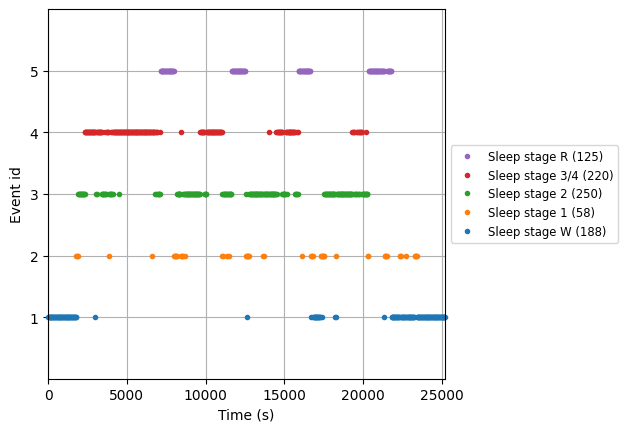
\includegraphics[width=0.60\textwidth]{img/paper_2/sleep event.PNG}
	\caption{Event Mapping Plot}
	\label{fig:lstm_accuracy}
\end{figure}


\subsection{Modeling Approach}

We implemented and evaluated several machine learning and deep learning architectures for the classification task. One of the core models used is the \textbf{Deep Neural Network (DNN)}, designed as a fully connected feedforward architecture suitable for non-sequential input.

\subsubsection{Deep Neural Network (DNN)}

The DNN consists of an input layer followed by three fully connected (\texttt{Dense}) layers comprising \textbf{128}, \textbf{64}, and \textbf{32} neurons respectively. Each layer employs the \textbf{ReLU} activation function to introduce non-linearity. To mitigate overfitting, \textbf{Dropout layers} with a dropout rate of \textbf{0.2} were interleaved between each dense layer. The final output layer uses a \textbf{Softmax} activation to produce class probabilities for the five sleep stages.




\section{Dataset Information}


ensure efficient implementation and reproducibility, this research adheres to a well-structured computational framework, including consistent system configuration, version control, and the integration of essential libraries for data processing and deep learning tasks. The experiments were conducted on both Windows and Linux operating systems using an \textbf{Intel Core i5 11th Gen} processor (with \textit{Iris Xe Graphics} and a clock speed of \textbf{3.9 GHz}). The programming environment was built with \textbf{Python version 3.13.1}, managed via the \texttt{pip} package installer.

The study utilized the \textbf{Sleep-EDF} dataset, which contains EEG recordings and corresponding hypnograms for sleep stage classification. Prior to model training, the dataset was preprocessed into uniform, fixed-length segments. The dataset is publicly available at: \url{https://www.physionet.org/content/sleep-edf/1.0.0/}.

For project collaboration and version control, \textbf{GitHub} was employed, with the full implementation accessible at: \url{https://github.com/tanmay007thor/ContraWR}.

Several key libraries were used throughout the development pipeline:
\begin{itemize}
	\item \textbf{NumPy (2.2.2)} – Numerical computations
	\item \textbf{scikit-learn (1.6.1)} – Machine learning utilities
	\item \textbf{imbalanced-learn (0.13.0)} – Handling class imbalance (SMOTE)
	\item \textbf{MNE (1.9.0)} – EEG signal processing
	\item \textbf{TensorFlow/Keras (2.16.1)} – Deep learning model implementation
	\item \textbf{Matplotlib (3.10.0)} and \textbf{Seaborn (0.13.2)} – Data visualization
\end{itemize}

This setup ensures smooth execution of machine learning and deep learning models, including BiLSTM and other architectures, for automating sleep stage classification.



\section{Preprocessing Techniques}

To ensure consistency in the input data, all recordings were resampled to a \textbf{100 Hz} sampling frequency. Each signal was segmented into \textbf{30-second epochs}, resulting in \textbf{3000 time steps per sample}. These samples were stored in \texttt{PKL} (Pickle) format, each approximately \textbf{48 KB} in size, enabling efficient storage and fast access, particularly beneficial for edge device deployment.

Each sample consisted of input-output pairs: the inputs ($X$) included two EEG channels—\textbf{FPZ-CZ} and \textbf{PZ-OZ}—while the labels ($Y$) represented the corresponding sleep stages. The stages were categorized into five classes: \textbf{Wake, N1, N2, N3,} and \textbf{REM}. To streamline processing, raw labels were mapped to a standardized class format.




\section{Model Architecture and Learning Framework}


\subsubsection{Deep Neural Network (DNN)}

A Deep Neural Network (DNN) is a type of multilayer feedforward architecture composed of successive fully connected layers. In this model, the input layer is followed by three dense layers containing 128, 64, and 32 neurons respectively. Each dense layer uses the Rectified Linear Unit (ReLU) activation function to introduce non-linearity.

To improve generalization and prevent overfitting, dropout layers with a dropout rate of 0.2 are inserted between the dense layers. The final output layer employs a Softmax activation function to map the learned features to the five target sleep stages: Wake, N1, N2, N3, and REM.

\begin{table}[H]
	\centering
	\caption{Architecture of the Deep Neural Network}
	\label{tab:nn_architecture}
	\begin{tabular}{lcc}
		\hline
		\textbf{Layer Type} & \textbf{Units} & \textbf{Activation Function} \\
		\hline
		Input Layer         & \texttt{X\_train}          & - \\
		Dense Layer         & 128                        & ReLU \\
		Dropout Layer       & -                          & 0.2 (Dropout Rate) \\
		Dense Layer         & 64                         & ReLU \\
		Dropout Layer       & -                          & 0.2 (Dropout Rate) \\
		Dense Layer         & 32                         & ReLU \\
		Dropout Layer       & -                          & 0.2 (Dropout Rate) \\
		Output Layer        & Number of classes (e.g., 5) & Softmax \\
		\hline
	\end{tabular}
\end{table}

While DNNs are effective in extracting complex feature representations from EEG signals, they are inherently limited in modeling temporal dependencies due to their feedforward nature. This limits their standalone utility for time-series classification tasks like sleep staging.

\subsubsection{Forward Propagation}

Forward propagation computes the activations at each layer using the following equations:

\begin{align}
	z^{(l)} &= W^{(l)} a^{(l-1)} + b^{(l)} \\
	a^{(l)} &= \sigma(z^{(l)})
\end{align}

\noindent where:
\begin{itemize}
	\item \( z^{(l)} \) is the pre-activation (linear combination of inputs) at layer \( l \),
	\item \( a^{(l)} \) is the activation output at layer \( l \),
	\item \( W^{(l)} \) and \( b^{(l)} \) denote the weights and biases of layer \( l \),
	\item \( \sigma \) is the activation function (ReLU or Softmax depending on the layer).
\end{itemize}

\subsubsection{Backward Propagation}

During training, gradients of the loss function with respect to weights and biases are calculated using backpropagation. The process involves the following steps:

\begin{align}
	\delta^{(L)} &= \frac{\partial L}{\partial a^{(L)}} \odot \sigma'(z^{(L)}) \\
	\delta^{(l)} &= \left(W^{(l+1)}\right)^T \delta^{(l+1)} \odot \sigma'(z^{(l)}) \\
	\frac{\partial L}{\partial W^{(l)}} &= \delta^{(l)} \left(a^{(l-1)}\right)^T \\
	\frac{\partial L}{\partial b^{(l)}} &= \sum \delta^{(l)}
\end{align}

\noindent where:
\begin{itemize}
	\item \( \delta^{(l)} \) is the error signal at layer \( l \),
	\item \( \sigma'(z^{(l)}) \) is the derivative of the activation function,
	\item \( \frac{\partial L}{\partial W^{(l)}} \) and \( \frac{\partial L}{\partial b^{(l)}} \) are gradients used for weight and bias updates.
\end{itemize}

\subsubsection{Activation Functions}

The Softmax function is used in the output layer to produce class probabilities:

\begin{equation}
	\sigma(z_i) = \frac{e^{z_i}}{\sum_{j=1}^{N} e^{z_j}}
\end{equation}

\noindent where:
\begin{itemize}
	\item \( z_i \) is the input to the \( i^{th} \) output neuron,
	\item \( N \) is the number of output classes,
	\item The denominator ensures the outputs form a probability distribution summing to 1.
\end{itemize}

For hidden layers, the ReLU activation function is applied:

\begin{equation}
	f(x) = \max(0, x)
\end{equation}

\noindent where:
\begin{itemize}
	\item \( x \) is the input to the neuron,
	\item The function outputs \( x \) if \( x > 0 \), and 0 otherwise.
\end{itemize}


\subsubsection{Recurrent Neural Network (RNN)}

Recurrent Neural Networks (RNNs) are specifically designed for modeling sequential data by incorporating feedback connections, allowing them to retain information across time steps. This architecture is well-suited for EEG signal analysis due to its ability to capture temporal dependencies.

In the proposed model, two RNN layers are employed: the first with 128 units and the second with 64 units, both using the Tanh activation function. These layers process sequential inputs while maintaining internal memory of past computations.

\begin{table}[!h]
	\centering
	\caption{Recurrent Neural Network Architecture for Sleep Stage Classification}
	\label{tab:rnn_architecture}
	\begin{tabular}{lcc}
		\hline
		\textbf{Layer Type} & \textbf{Units} & \textbf{Activation Function} \\
		\hline
		Input Layer         & \texttt{X\_train}          & - \\
		RNN Layer 1         & 128                        & Tanh \\
		Dropout Layer       & -                          & 0.2 (Dropout Rate) \\
		RNN Layer 2         & 64                         & Tanh \\
		Dropout Layer       & -                          & 0.2 (Dropout Rate) \\
		Dense Layer         & 64                         & ReLU \\
		Dropout Layer       & -                          & 0.2 (Dropout Rate) \\
		Dense Layer         & 32                         & ReLU \\
		Dropout Layer       & -                          & 0.2 (Dropout Rate) \\
		Output Layer        & Number of classes (e.g., 5) & Softmax \\
		\hline
	\end{tabular}
\end{table}

Dropout layers with a 0.2 rate are introduced after each RNN and dense layer to mitigate overfitting. The dense layers, activated using ReLU, help to refine temporal features extracted by the RNN layers. The final classification is performed by a Softmax-activated output layer corresponding to the target sleep stages.

Although RNNs are effective for learning short-term dependencies in sequential EEG data, they are prone to issues such as vanishing gradients, which can hinder the learning of long-range patterns.

The operation of an RNN cell at each time step \( t \) is mathematically represented as:

\begin{equation}
	h_t = \tanh(W_h h_{t-1} + W_x x_t + b_h)
\end{equation}

\noindent where:
\begin{itemize}
	\item \( h_t \) is the hidden state at time step \( t \),
	\item \( x_t \) is the input at time step \( t \),
	\item \( W_h \) and \( W_x \) are the recurrent and input weight matrices, respectively,
	\item \( b_h \) is the bias vector,
	\item \( \tanh \) is the hyperbolic tangent activation function.
\end{itemize}



\subsubsection{Long Short-Term Memory (LSTM)}

Long Short-Term Memory (LSTM) networks extend traditional RNNs by incorporating memory cells and gating mechanisms, enabling them to retain long-term dependencies in sequential data. This makes them particularly effective for time-series applications like EEG-based sleep stage classification.

The proposed LSTM architecture includes two stacked LSTM layers with 128 and 64 units, respectively, both using the Tanh activation function to handle nonlinear temporal patterns in the data. To prevent overfitting, dropout layers with a rate of 0.2 are placed after each LSTM and dense layer.

\begin{table}[H]
	\centering
	\caption{LSTM Neural Network Architecture for Sleep Stage Classification}
	\label{tab:lstm_architecture}
	\begin{tabular}{lcc}
		\hline
		\textbf{Layer Type} & \textbf{Units} & \textbf{Activation Function} \\
		\hline
		Input Layer         & \texttt{X\_train}           & - \\
		LSTM Layer 1        & 128                         & Tanh \\
		Dropout Layer       & -                           & 0.2 (Dropout Rate) \\
		LSTM Layer 2        & 64                          & Tanh \\
		Dropout Layer       & -                           & 0.2 (Dropout Rate) \\
		Dense Layer         & 64                          & ReLU \\
		Dropout Layer       & -                           & 0.2 (Dropout Rate) \\
		Dense Layer         & 32                          & ReLU \\
		Dropout Layer       & -                           & 0.2 (Dropout Rate) \\
		Output Layer        & Number of classes (e.g., 5) & Softmax \\
		\hline
	\end{tabular}
\end{table}

The dense layers following the LSTM blocks (with 64 and 32 units) refine the extracted temporal features using ReLU activations. The final output layer uses the Softmax function to perform multi-class classification of sleep stages. LSTM models are particularly advantageous in capturing long-range dependencies and complex temporal dynamics, thus often outperforming simple RNNs for EEG sequence modeling.

LSTM cells operate through a series of gating mechanisms that regulate the flow of information. The key equations governing an LSTM cell at time step \( t \) are:

\begin{align}
	f_t &= \sigma(W_f x_t + U_f h_{t-1} + b_f) \quad \text{(Forget Gate)} \\
	i_t &= \sigma(W_i x_t + U_i h_{t-1} + b_i) \quad \text{(Input Gate)} \\
	\tilde{c}t &= \tanh(W_c x_t + U_c h{t-1} + b_c) \quad \text{(Candidate Cell State)} \\
	c_t &= f_t \odot c_{t-1} + i_t \odot \tilde{c}_t \quad \text{(Cell State Update)} \\
	o_t &= \sigma(W_o x_t + U_o h_{t-1} + b_o) \quad \text{(Output Gate)} \\
	h_t &= o_t \odot \tanh(c_t) \quad \text{(Hidden State Update)}
\end{align}

\noindent where:
\begin{itemize}
	\item \( f_t, i_t, o_t \) represent the forget, input, and output gates, respectively.
	\item \( \tilde{c}_t \) is the candidate cell state.
	\item \( c_t \) is the updated memory cell state.
	\item \( h_t \) is the hidden state at time \( t \).
	\item \( \sigma \) denotes the sigmoid activation function.
	\item \( \odot \) represents element-wise multiplication.
	\item \( W, U, b \) are the learned weight matrices and biases.
\end{itemize}


\subsubsection{Bidirectional Long Short-Term Memory (Bi-LSTM)}

The Bidirectional Long Short-Term Memory (Bi-LSTM) network enhances the LSTM model by processing input sequences in both forward and backward directions, enabling the model to learn context from both past and future data. This bidirectional approach improves the model's ability to capture dependencies in temporal data, making it highly effective for tasks such as EEG-based sleep stage classification.

The architecture consists of two bidirectional LSTM layers with 128 and 64 units, respectively, both utilizing the Tanh activation function. Dropout layers (with a rate of 0.2) are applied after each LSTM layer to prevent overfitting. Following the bidirectional LSTM layers, dense layers with 64 and 32 units, using ReLU activation, are added to refine the learned features before the final classification layer, which uses the Softmax activation to classify the sleep stages.

\begin{table}[!h]
	\centering
	\caption{Bidirectional LSTM Neural Network Architecture for Sleep Stage Classification}
	\label{tab:bi_lstm_architecture}
	\begin{tabular}{lcc}
		\hline
		\textbf{Layer Type} & \textbf{Units} & \textbf{Activation Function} \\
		\hline
		Input Layer         & \texttt{X\_train}            & - \\
		Bi-LSTM Layer 1     & 128                          & Tanh \\
		Dropout Layer       & -                            & 0.2 (Dropout Rate) \\
		Bi-LSTM Layer 2     & 64                           & Tanh \\
		Dropout Layer       & -                            & 0.2 (Dropout Rate) \\
		Dense Layer         & 64                           & ReLU \\
		Dropout Layer       & -                            & 0.2 (Dropout Rate) \\
		Dense Layer         & 32                           & ReLU \\
		Dropout Layer       & -                            & 0.2 (Dropout Rate) \\
		Output Layer        & Number of classes (e.g., 5)  & Softmax \\
		\hline
	\end{tabular}
\end{table}

Bi-LSTM networks are particularly well-suited for EEG-based sleep stage classification, as they allow the model to capture both past and future dependencies in the EEG signal, leading to improved accuracy in detecting sleep patterns.

The Bi-LSTM model processes input sequences in both forward and backward directions, maintaining two hidden states for each timestep. The key equations describing the forward and backward passes are:

\begin{align}
	\overrightarrow{h}t &= \text{LSTM}(x_t, \overrightarrow{h}{t-1}) \\
	\overleftarrow{h}t &= \text{LSTM}(x_t, \overleftarrow{h}{t+1}) \\
	h_t &= [\overrightarrow{h}_t; \overleftarrow{h}_t]
\end{align}

where:
\begin{itemize}
	\item \( \overrightarrow{h}_t \) is the forward LSTM hidden state at time step \( t \).
	\item \( \overleftarrow{h}_t \) is the backward LSTM hidden state at time step \( t \).
	\item \( h_t \) is the concatenated hidden state, combining both forward and backward states, used for final predictions.
\end{itemize}








\section{Results and Evaluation}





\subsection{Neural Network (NN) Model}

\begin{figure}[H]
	\centering
	\begin{minipage}{0.66\textwidth}
		\centering
		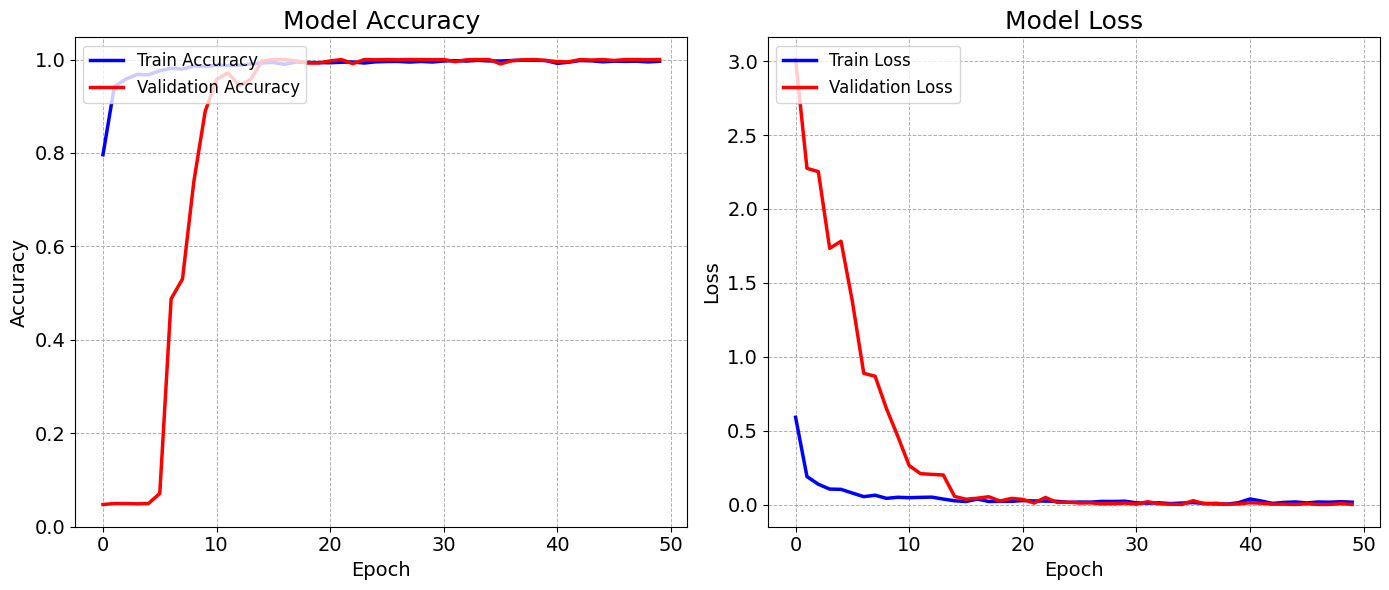
\includegraphics[width=\linewidth]{img/paper_2/deeplearning.png}
		\caption{Neural Network Accuracy and Loss Comparison}
		\label{fig:nn_accuracy}
	\end{minipage}
	\hfill
	\begin{minipage}{0.33\textwidth}
		\centering
		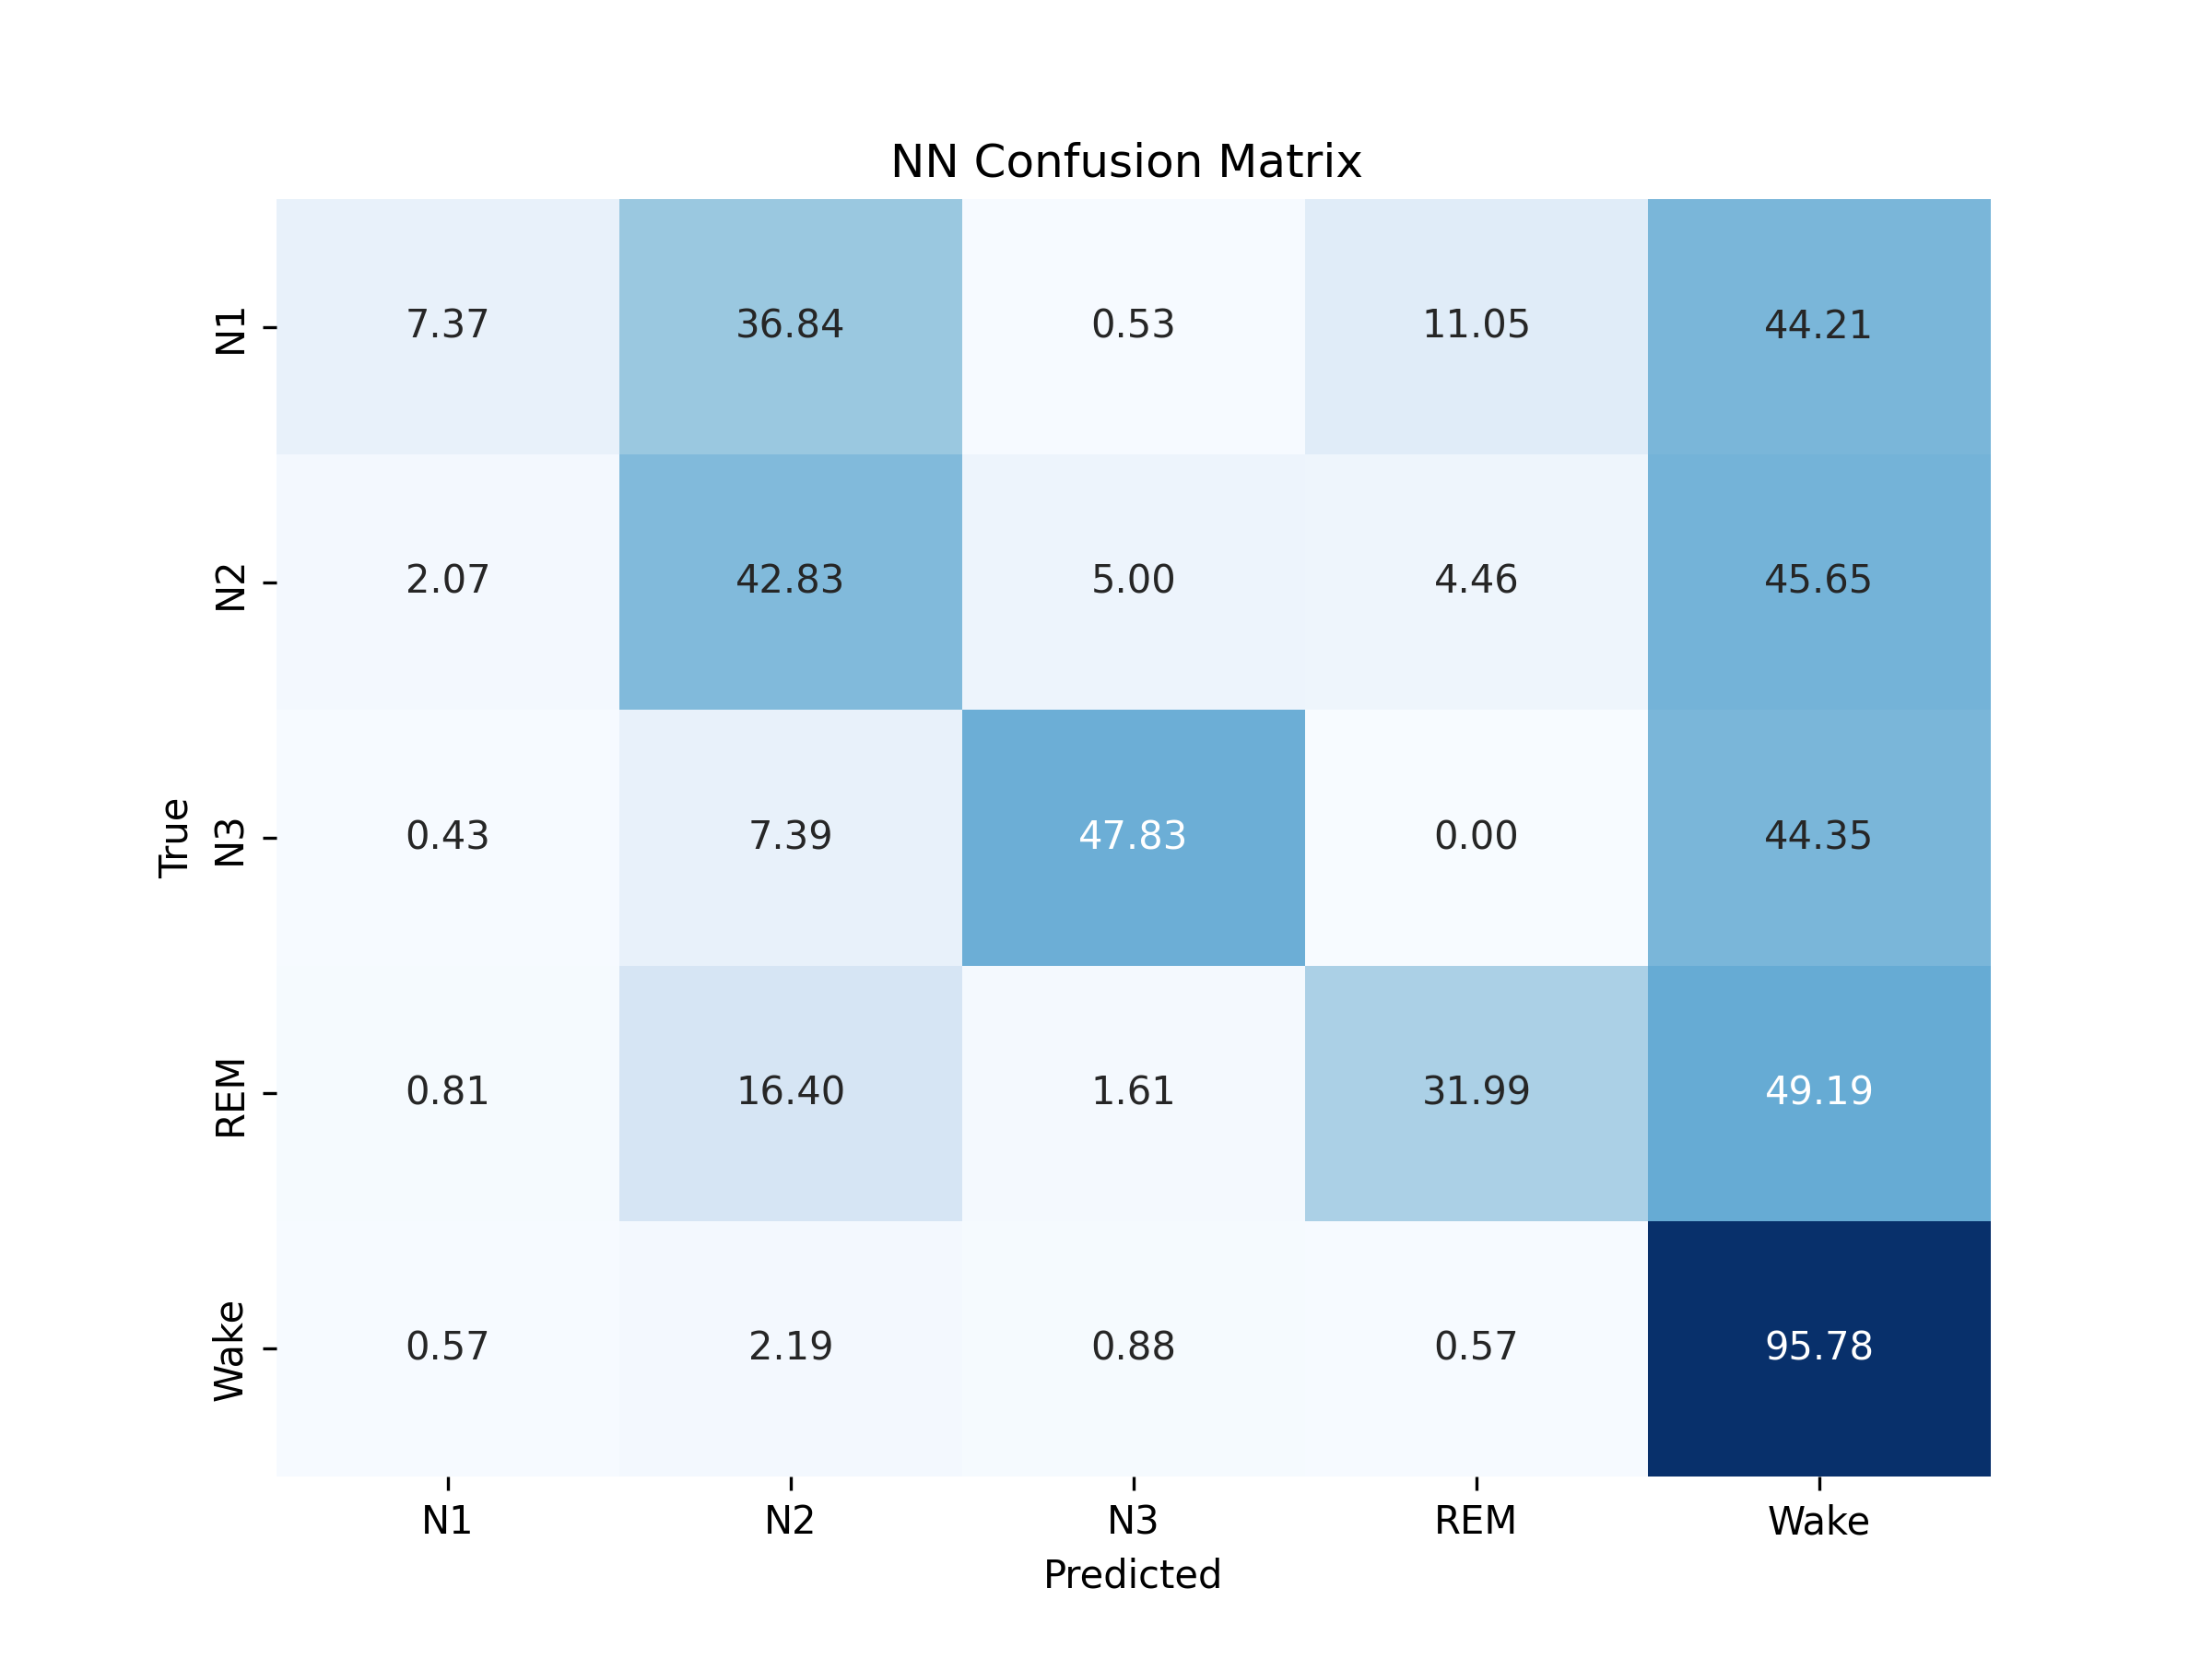
\includegraphics[width=\linewidth]{img/paper_2/NN_cm.png}
		\caption{Neural Network Confusion Matrix}
		\label{fig:nn_cm}
	\end{minipage}
\end{figure}


\subsection{LSTM Model}

\begin{figure}[H]
	\centering
	\begin{minipage}{0.66\textwidth}
		\centering
		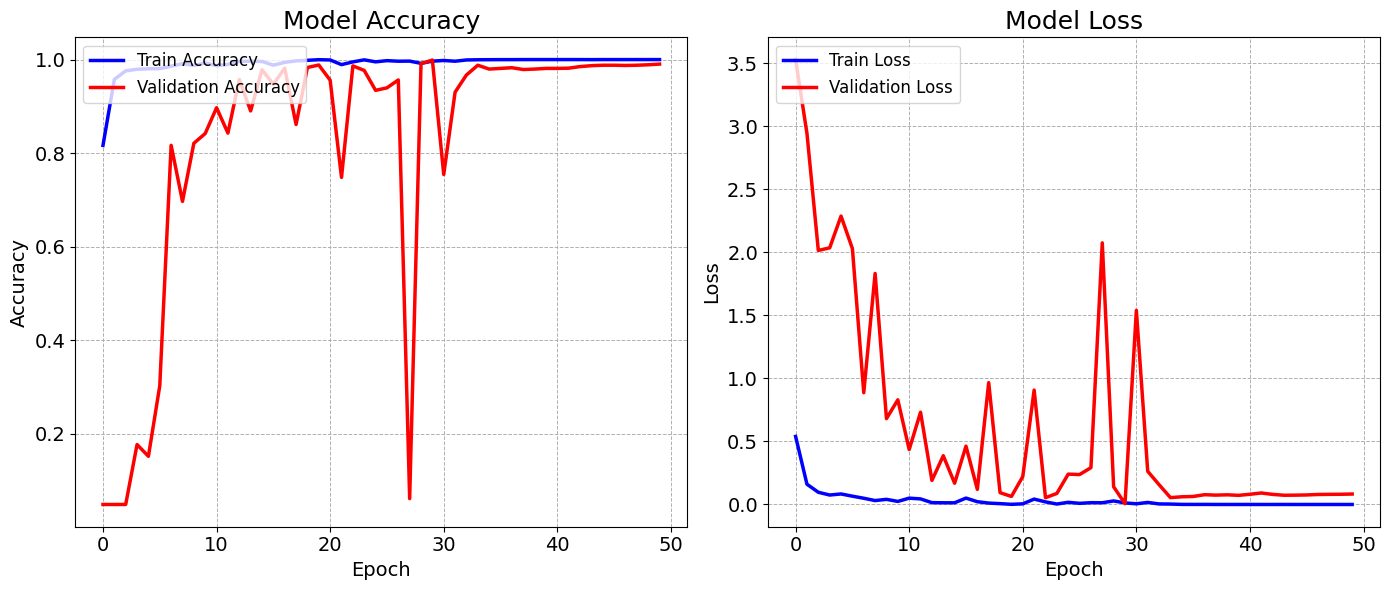
\includegraphics[width=\linewidth]{img/paper_2/lstm accuracy and loss plot.png}
		\caption{LSTM Accuracy and Loss Plot}
		\label{fig:lstm_accuracy}
	\end{minipage}
	\hfill
	\begin{minipage}{0.32\textwidth}
		\centering
		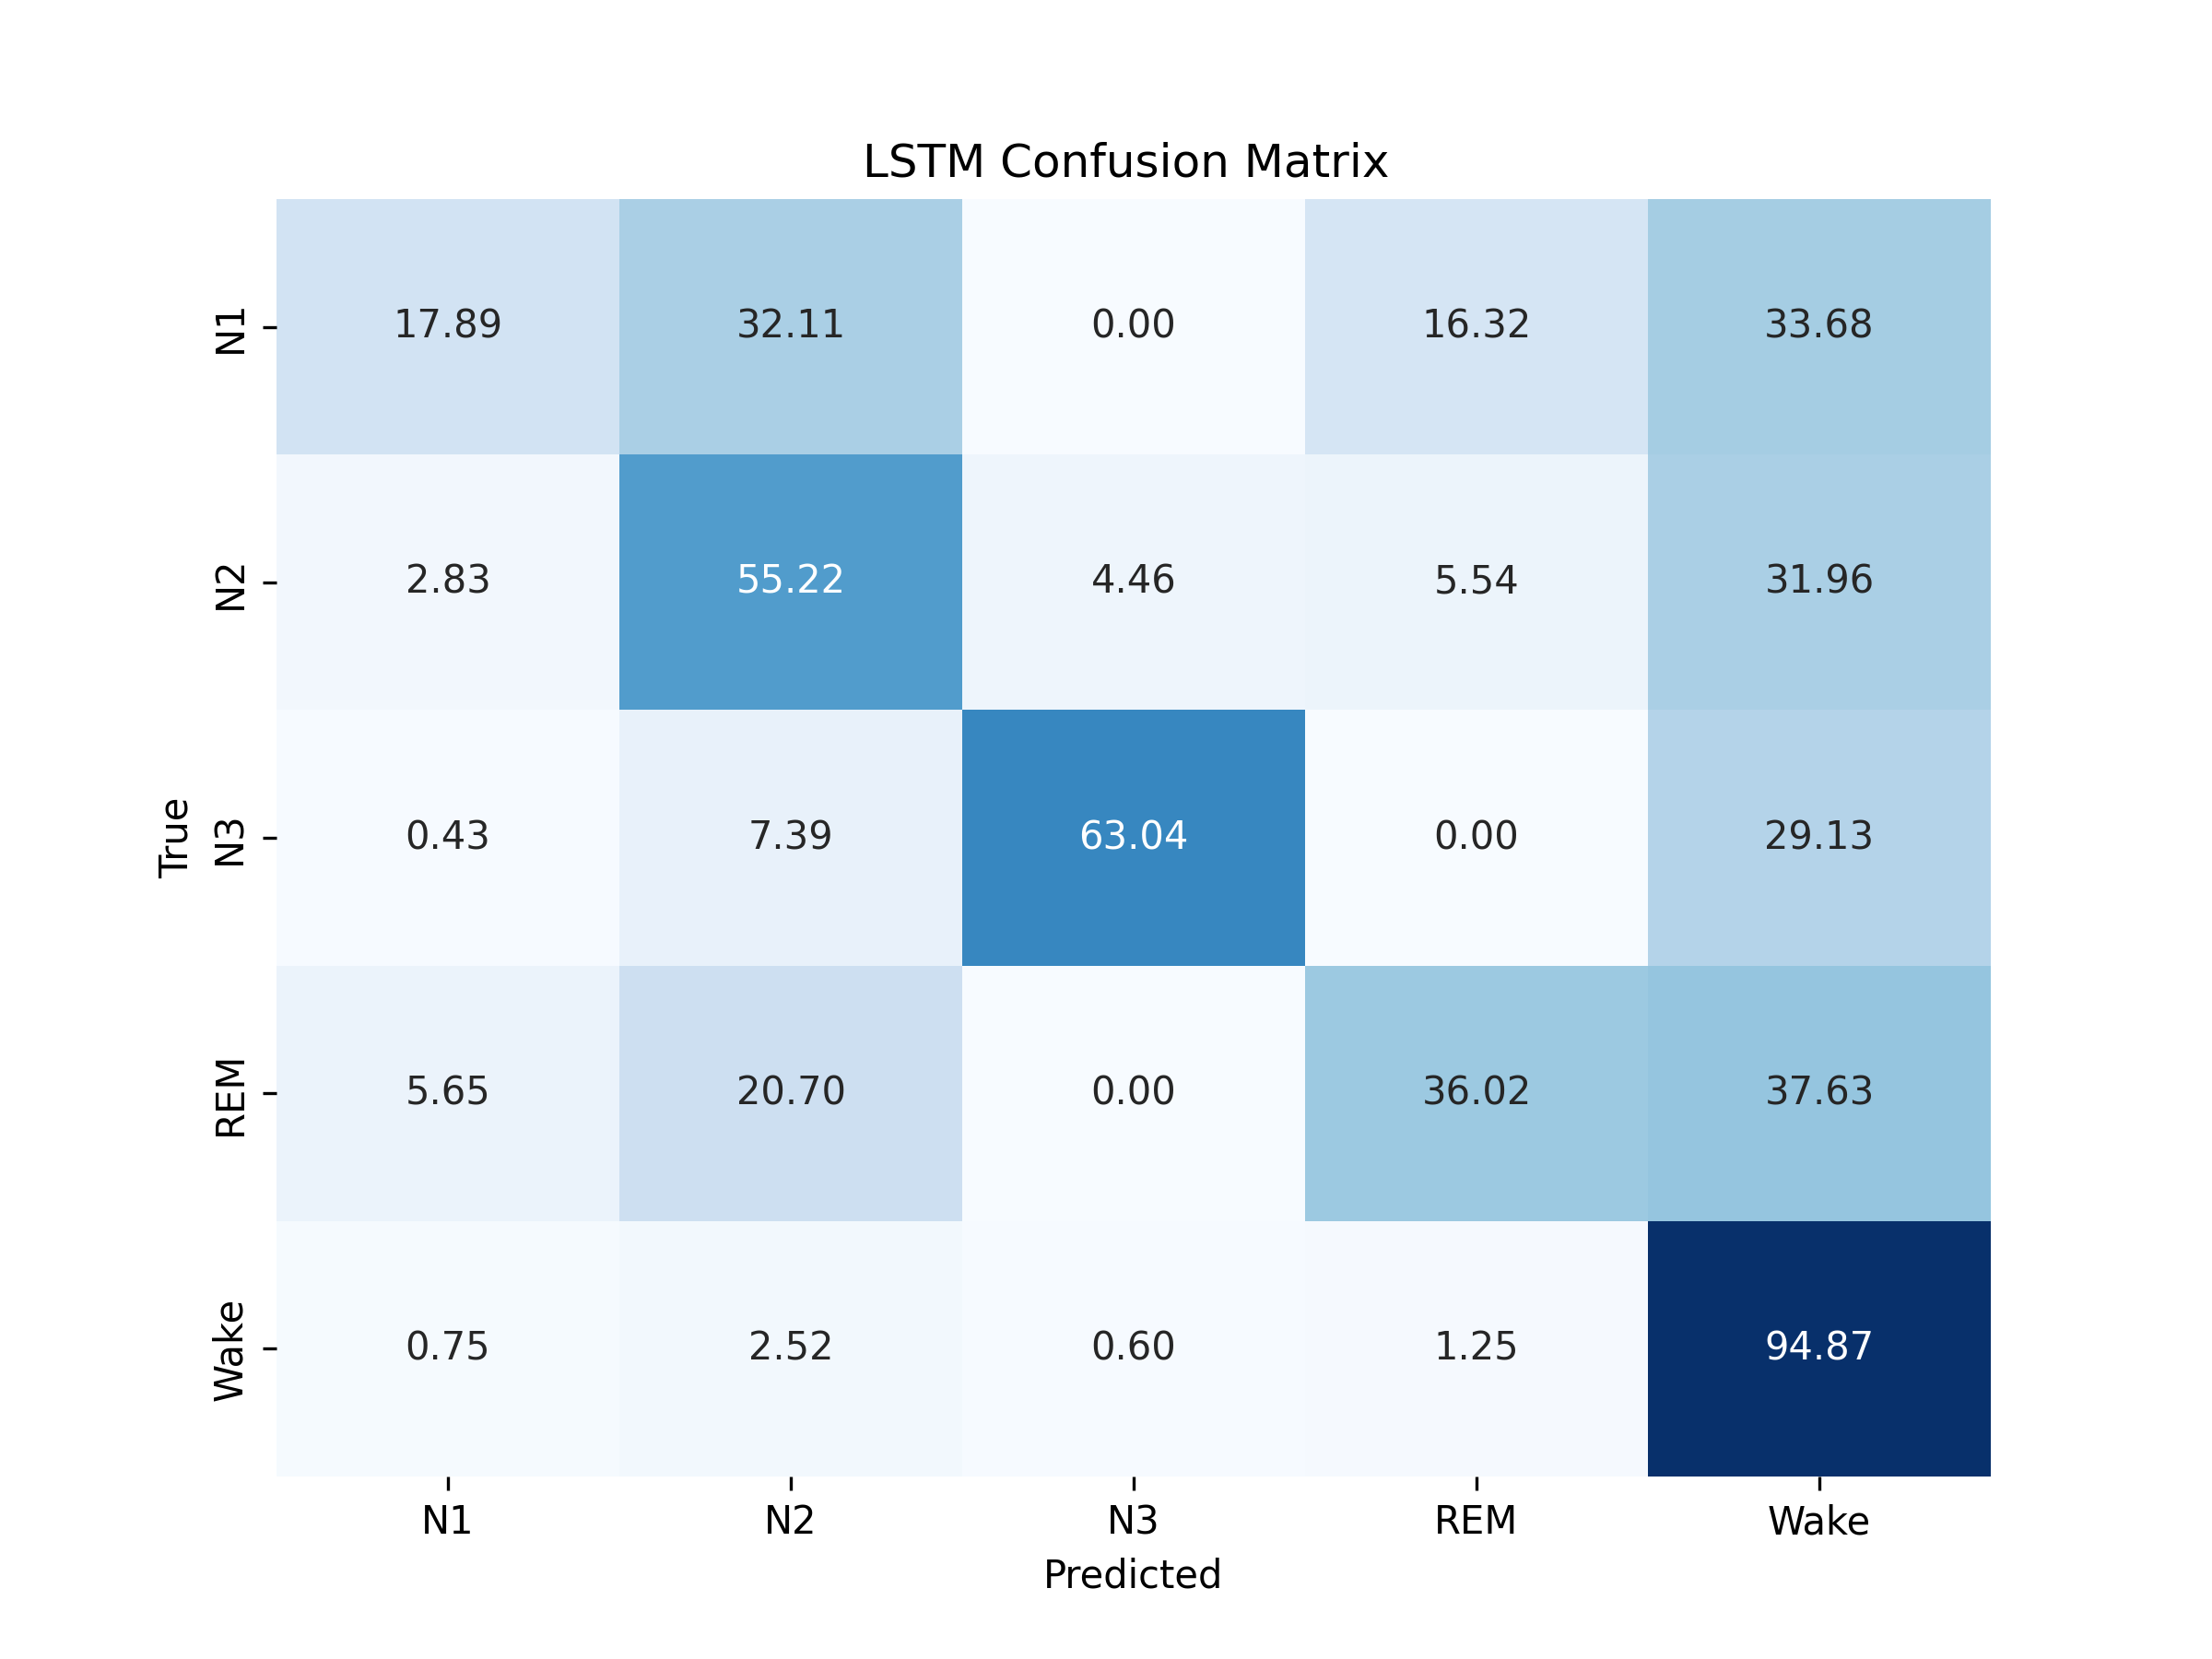
\includegraphics[width=\linewidth]{img/paper_2/LSTM_cm.png}
		\caption{LSTM Confusion Matrix}
		\label{fig:lstm_cm}
	\end{minipage}
\end{figure}


\subsection{RNN Model}

\begin{figure}[H]
	\centering
	\begin{minipage}{0.66\textwidth}
		\centering
		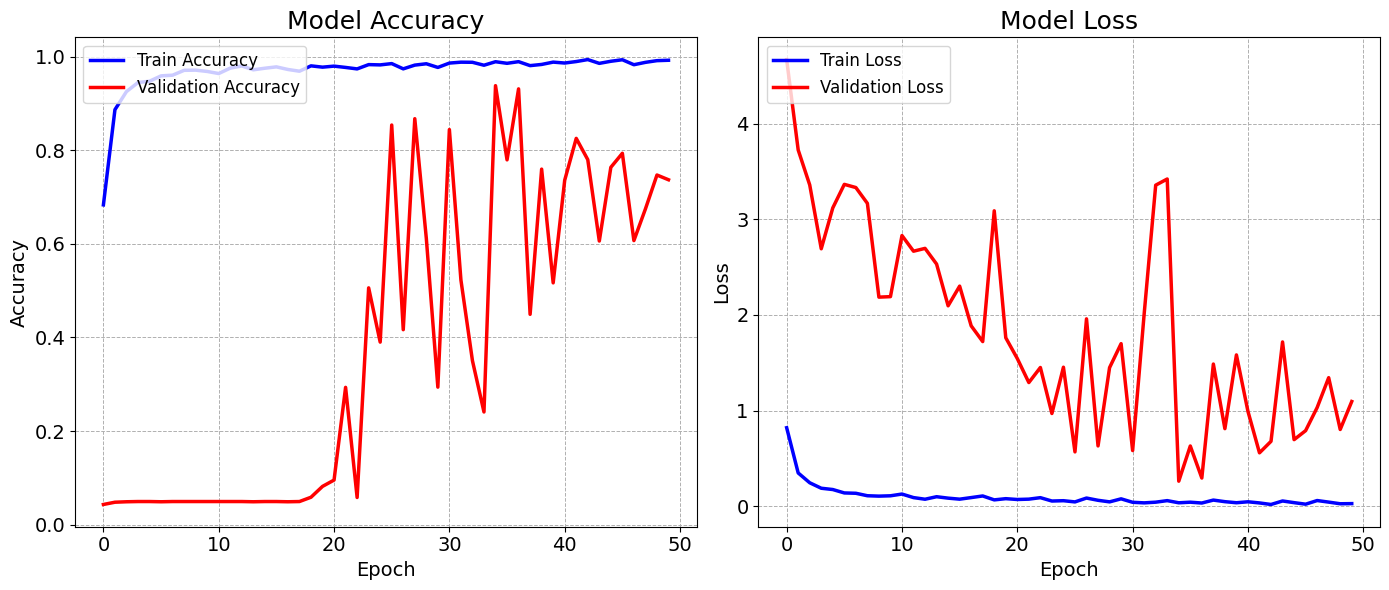
\includegraphics[width=\linewidth]{img/paper_2/Rnn Accuracy Plot.png}
		\caption{RNN Accuracy Plot}
		\label{fig:rnn_accuracy}
	\end{minipage}
	\hfill
	\begin{minipage}{0.32\textwidth}
		\centering
		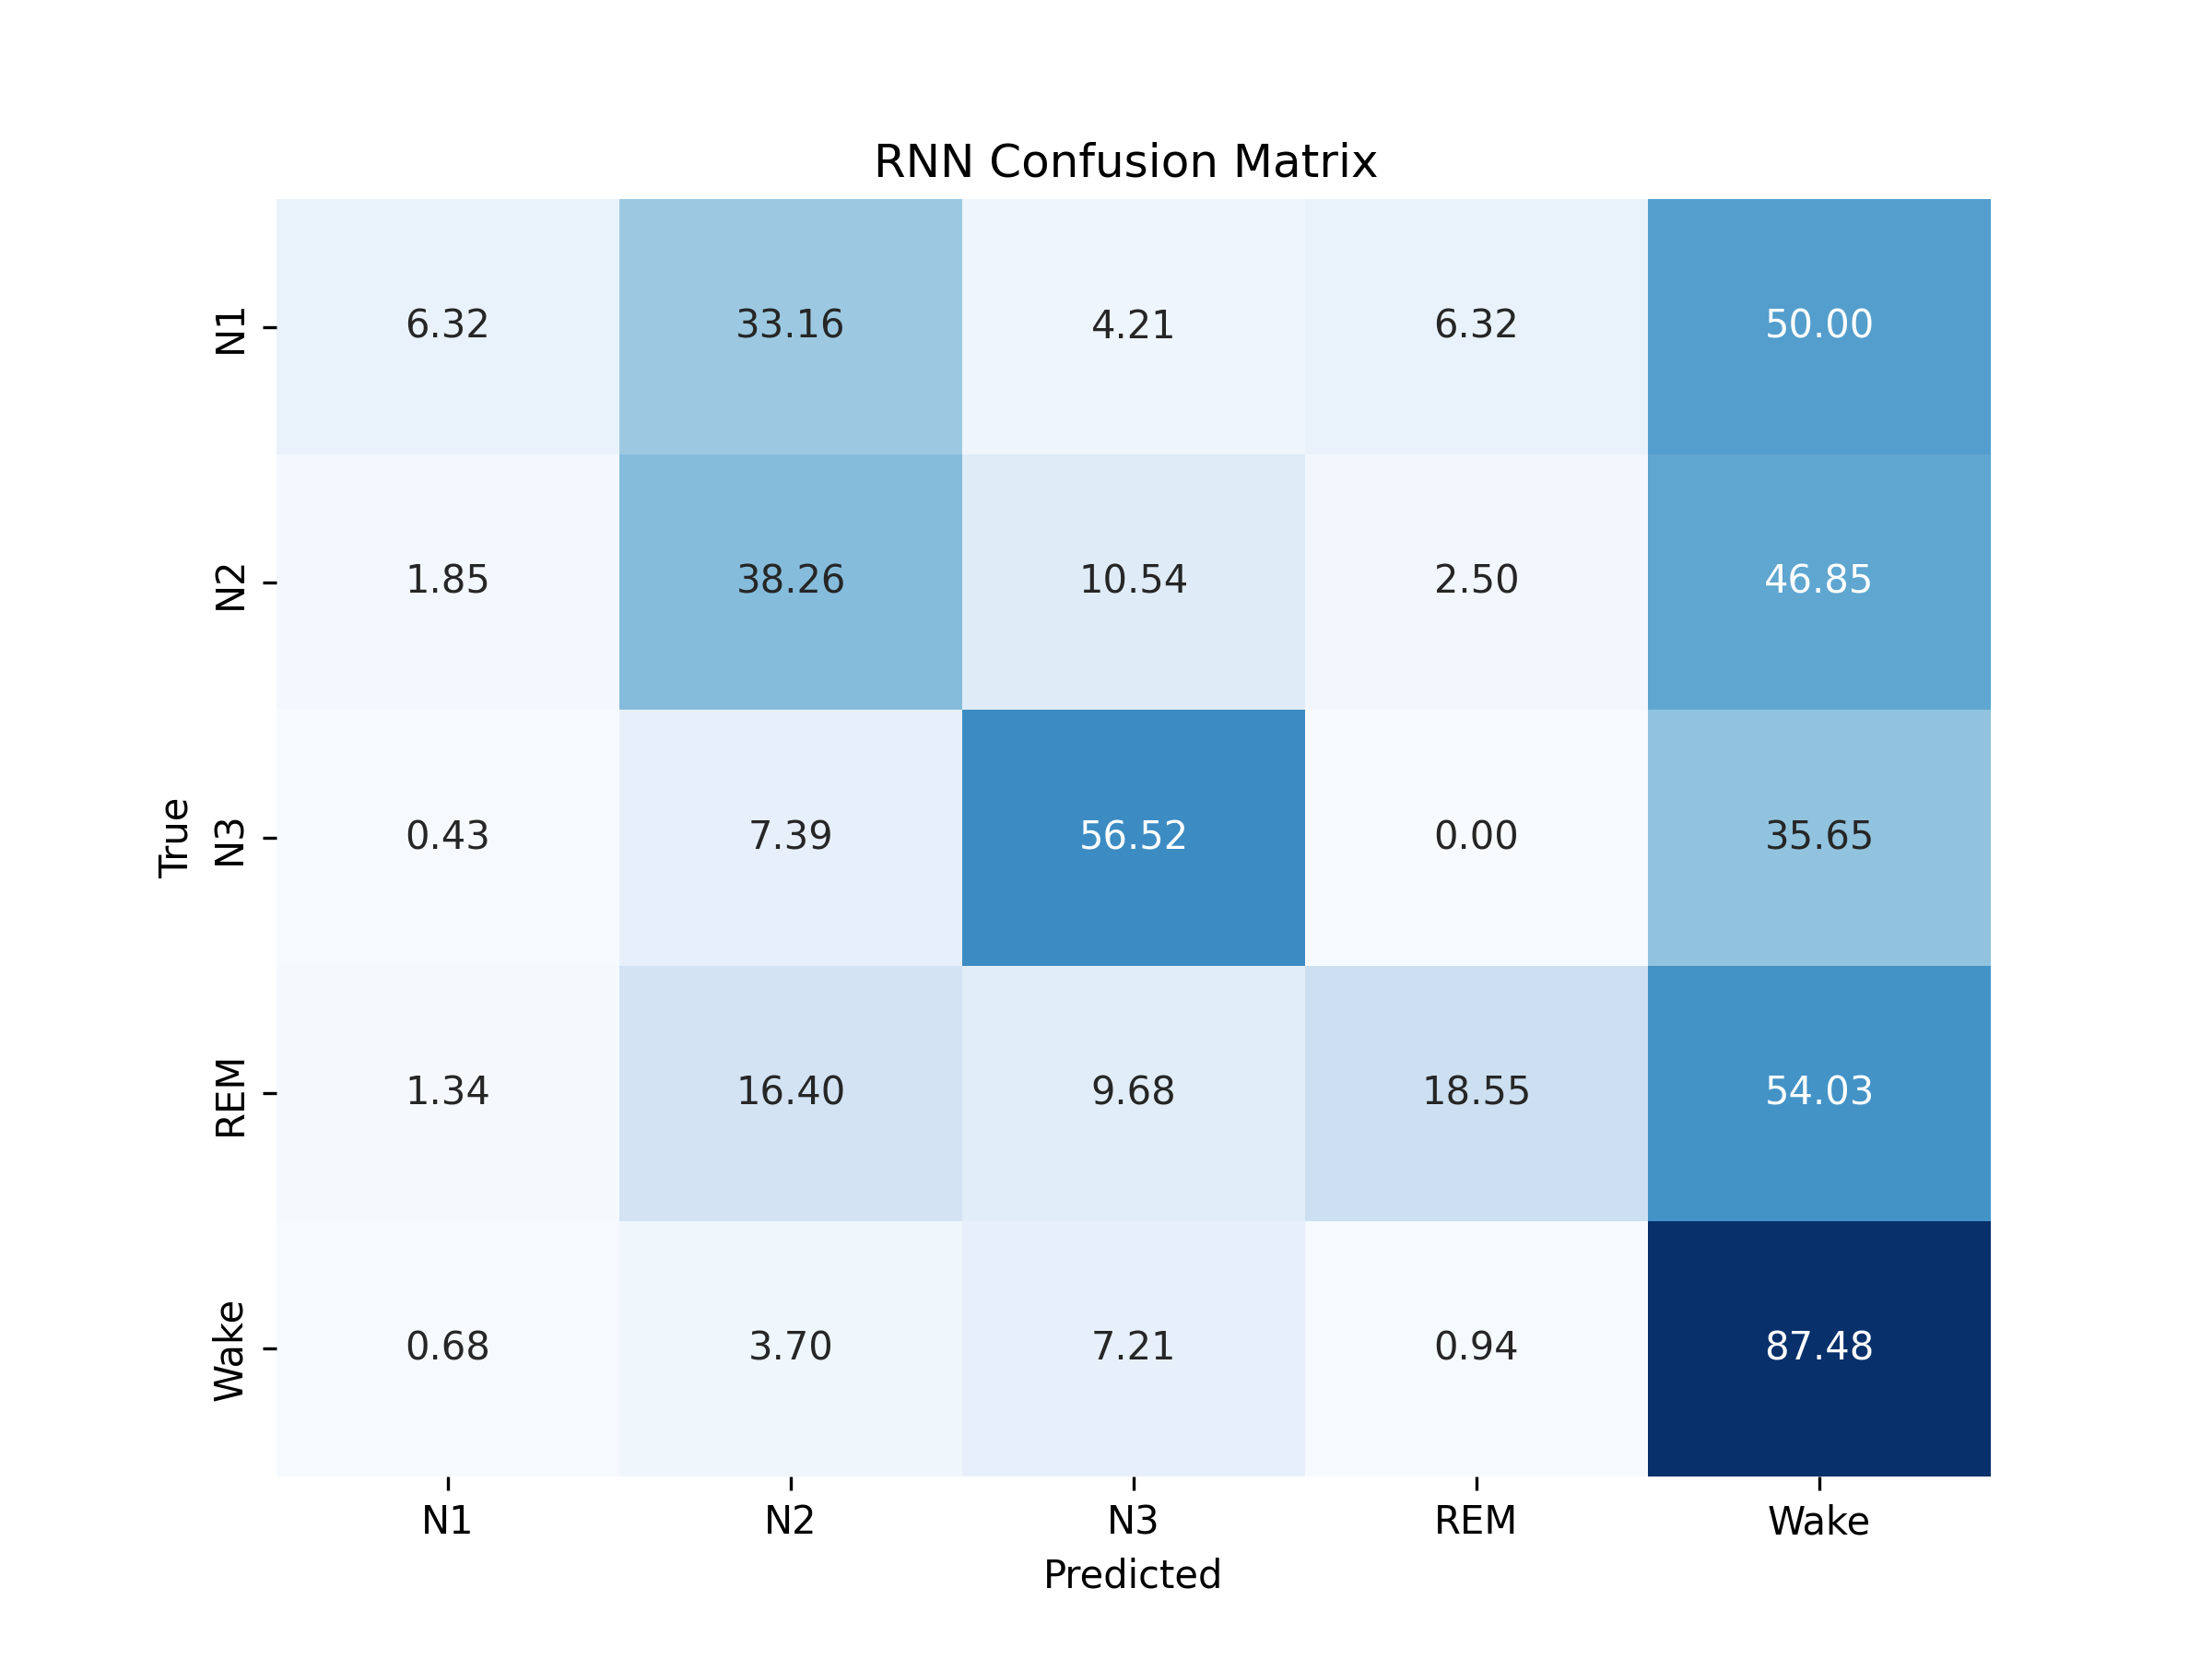
\includegraphics[width=\linewidth]{img/paper_2/RNN_cm.png}
		\caption{RNN Confusion Matrix}
		\label{fig:rnn_cm}
	\end{minipage}
\end{figure}


\subsection{BiLSTM Model}

\begin{figure}[H]
	\centering
	\begin{minipage}{0.66\textwidth}
		\centering
		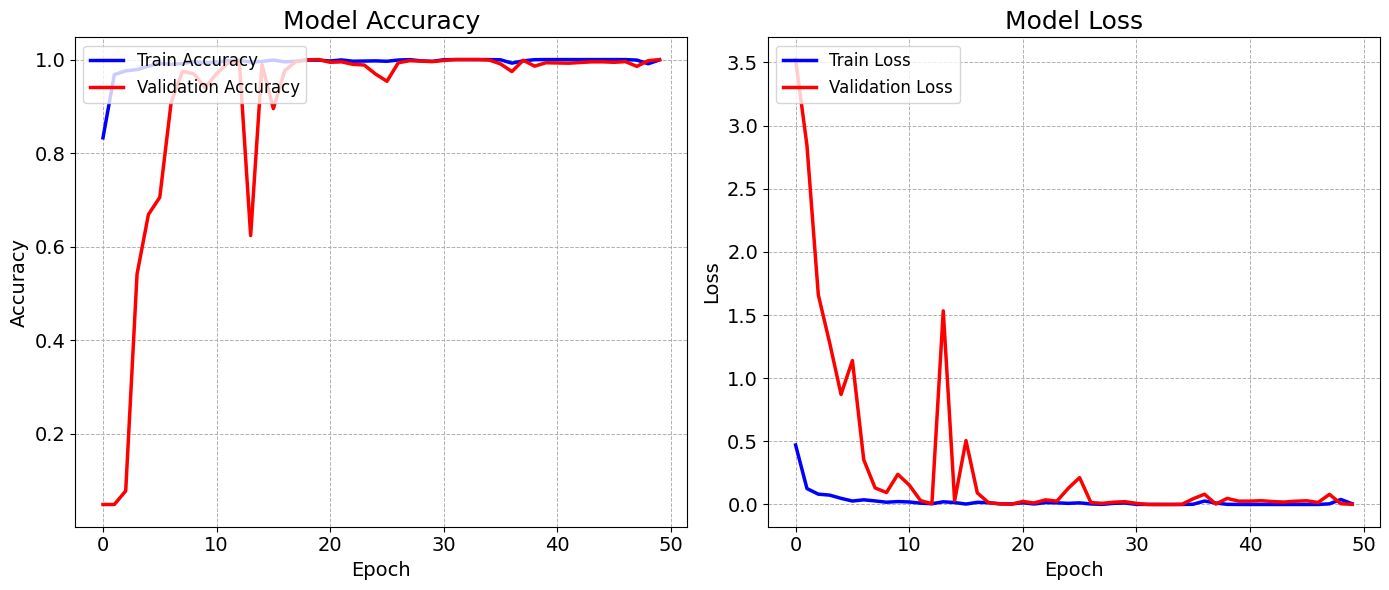
\includegraphics[width=\linewidth]{img/paper_2/BILSTM Accuaracy Plot.png}
		\caption{BiLSTM Accuracy Plot}
		\label{fig:bilstm_accuracy}
	\end{minipage}
	\hfill
	\begin{minipage}{0.32\textwidth}
		\centering
		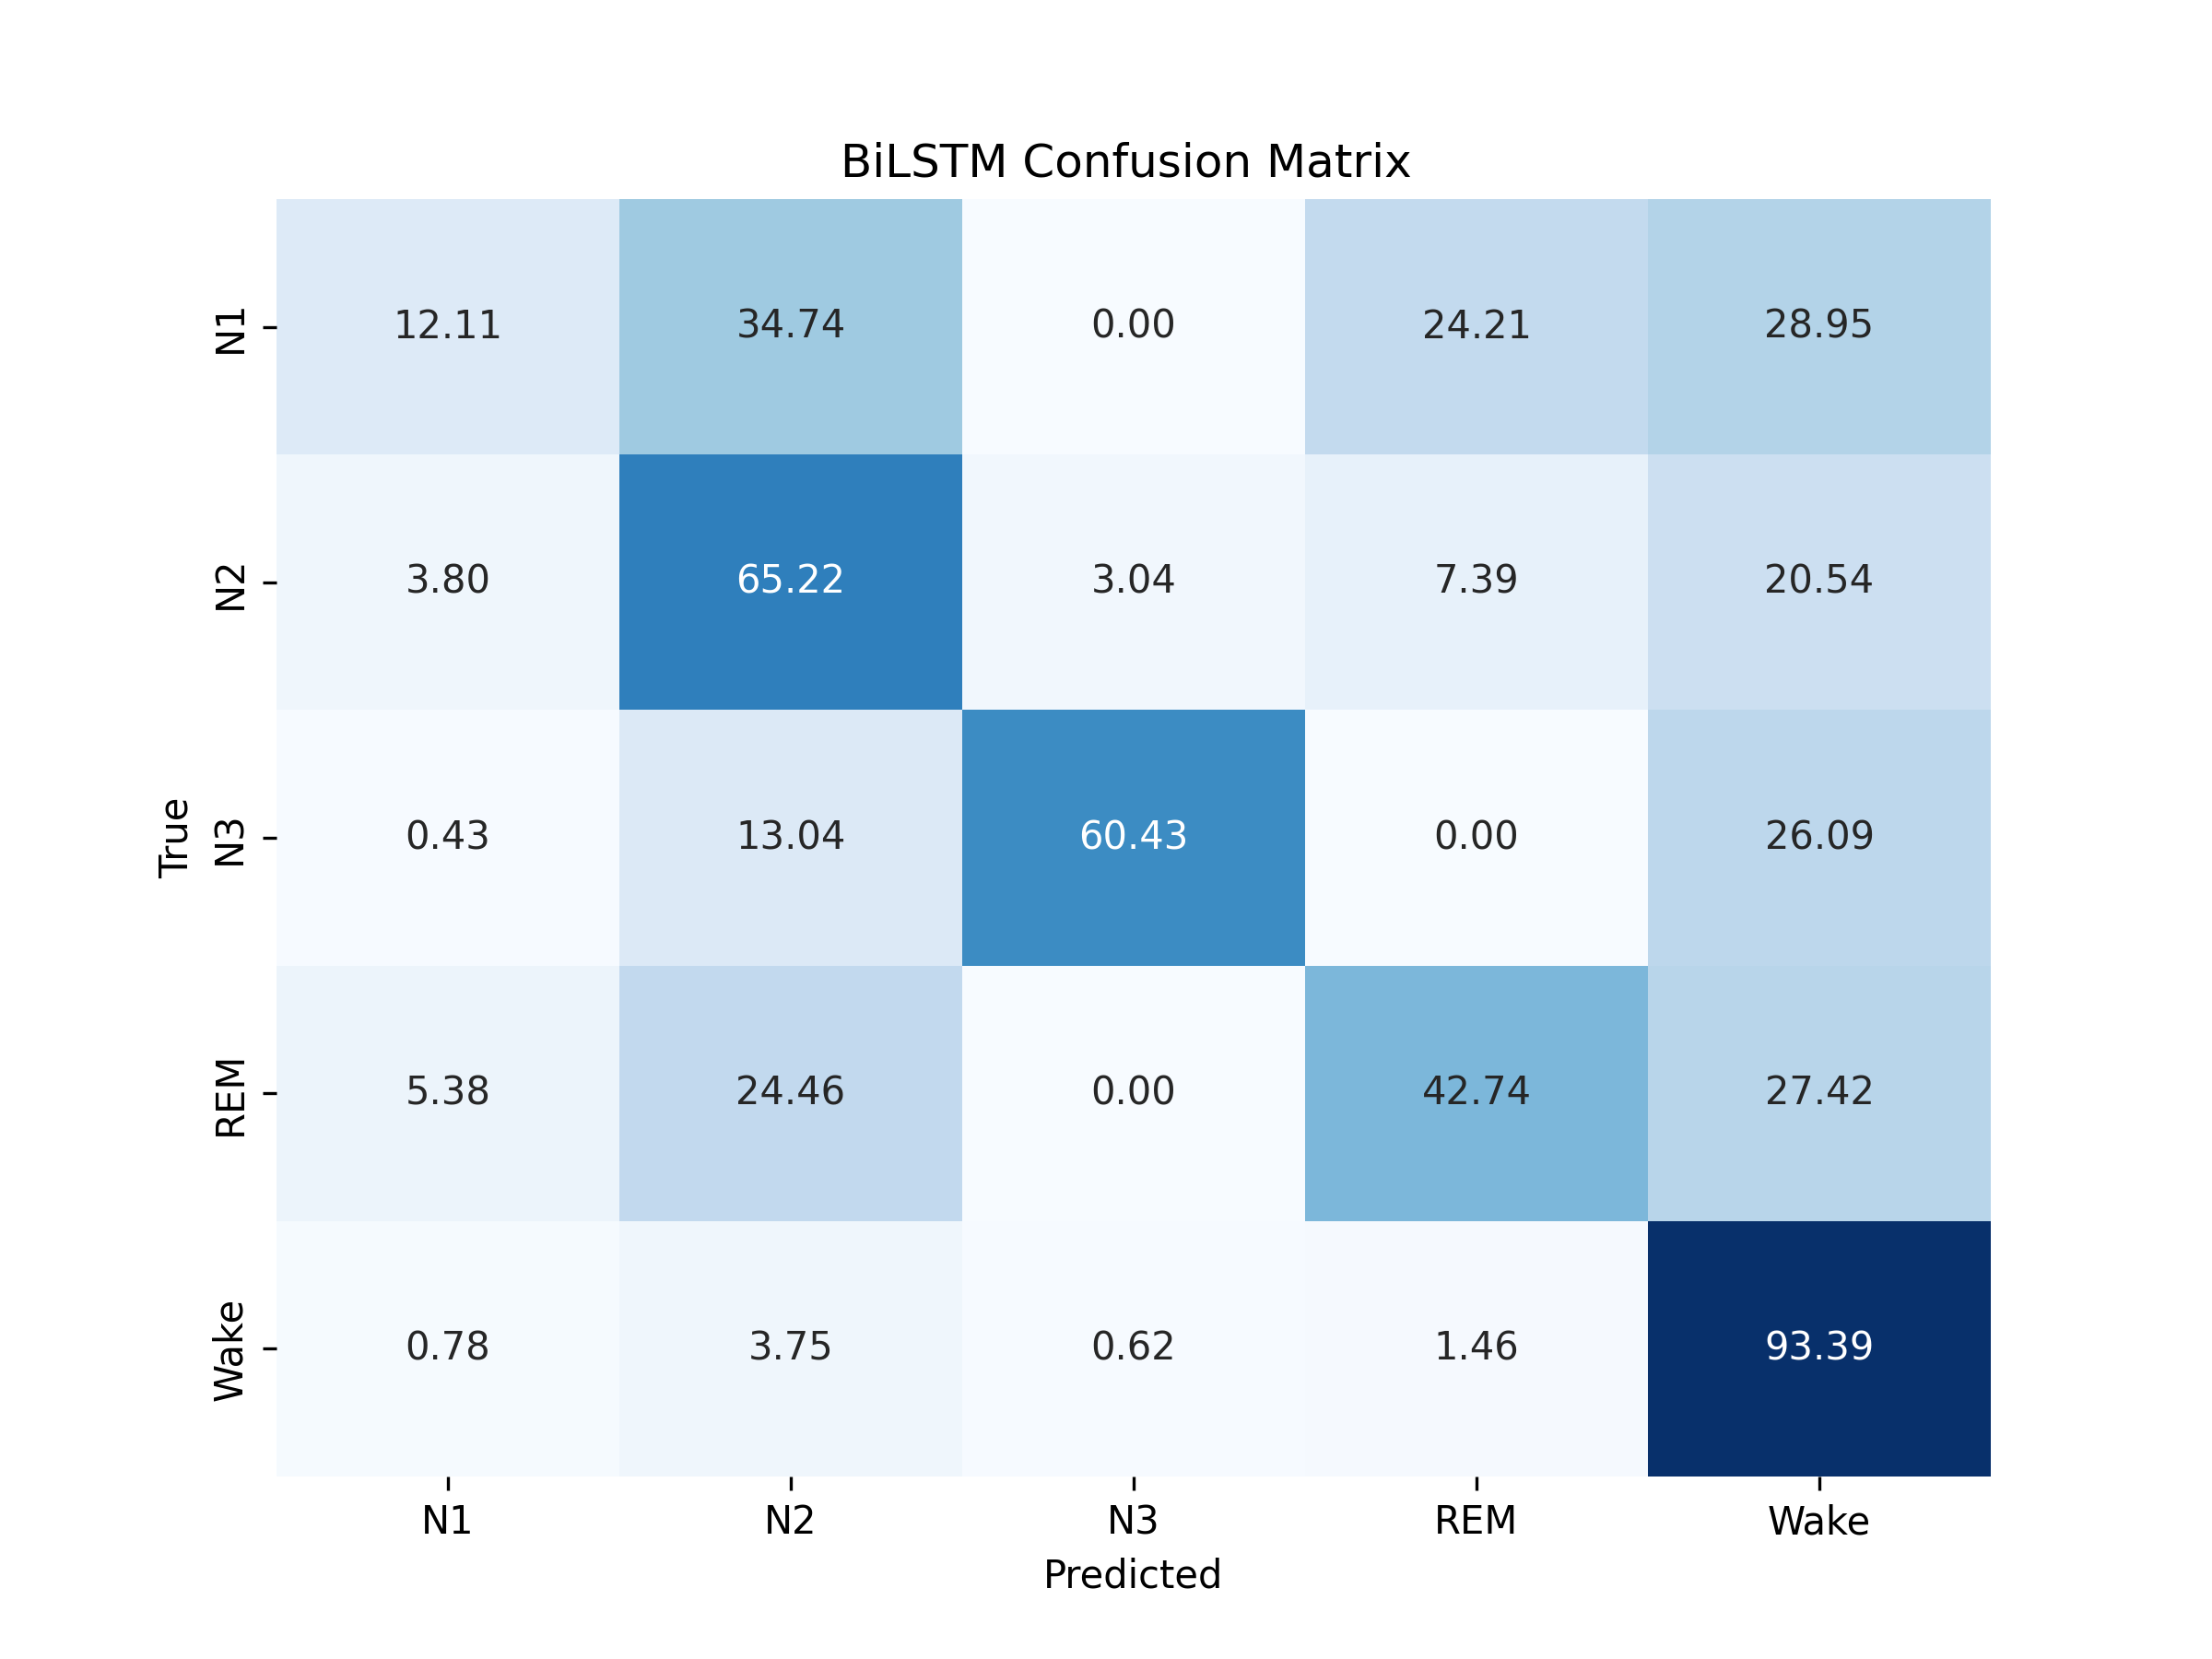
\includegraphics[width=\linewidth]{img/paper_2/BiLSTM_cm.png}
		\caption{BiLSTM Confusion Matrix}
		\label{fig:bilstm_cm}
	\end{minipage}
\end{figure}



\section{Comparison of Results}



This section presents a comparative analysis of multiple machine learning models applied to the sleep stage classification problem. The evaluation metrics considered include accuracy, weighted and macro averages of precision, recall, and F1-score.

\subsection{Testing  Models Overview}



\begin{table}[H]
	\centering
	\caption{Performance Comparison of Models}
	\label{tab:metrics_summary}
	\begin{tabular}{lcccccc}
		\hline
		\textbf{Model} & \textbf{Accuracy} & \textbf{Wgt. F1} & \textbf{Macro F1} & \textbf{Macro Prec.} & \textbf{Macro Rec.} \\
		\hline
		Random Forest          & \textbf{0.843} & \textbf{0.823} & 0.641 & \textbf{0.901} & 0.558 \\
		XGBoost                & \textbf{0.854} & \textbf{0.843} & 0.644 & \textbf{0.776} & 0.599 \\
		Neural Network         & \textbf{0.777} & \textbf{0.750} & 0.487 & 0.567 & 0.452 \\
		LSTM                   & \textbf{0.800} & \textbf{0.785} & 0.461 & 0.499 & 0.436 \\
		BiLSTM                 & \textbf{0.811} & \textbf{0.803} & 0.472 & 0.494 & 0.457 \\
		RNN                    & 0.706 & 0.690 & 0.332 & 0.381 & 0.345 \\
		AdaBoost               & 0.312 & 0.353 & 0.273 & 0.323 & 0.399 \\
		KNN (with PCA)         & 0.194 & 0.189 & 0.272 & 0.296 & 0.359 \\
		\hline
	\end{tabular}
\end{table}


\subsection{Discussion}

Among all the models tested, the \textbf{XGBoost classifier} achieved the highest overall accuracy (0.854) and weighted F1-score (0.843), narrowly outperforming the Random Forest model. While Random Forest achieved a slightly higher macro precision (0.901 vs. 0.776), its recall across minority classes such as N1 and REM was relatively lower.

The deep learning-based models (LSTM and BiLSTM) followed closely behind the tree-based models, with BiLSTM slightly outperforming LSTM (macro F1 of 0.472 vs. 0.461). The \textbf{Neural Network model}, although simpler, showed moderate performance (macro F1 of 0.487), better than AdaBoost and KNN.

\textbf{K-Nearest Neighbors (KNN)} and \textbf{AdaBoost} performed poorly in this context. KNN failed to handle the class imbalance effectively, leading to very low overall accuracy (0.194). AdaBoost performed slightly better but still struggled to generalize, especially for majority class (Wake) classification.

The \textbf{RNN model} had the lowest macro F1-score (0.332) among deep models, indicating potential vanishing gradient issues or insufficient context capture compared to LSTM-based architectures.

\subsection{Conclusion}

Tree-based ensemble methods (XGBoost, Random Forest) consistently outperformed others across all key metrics. Deep learning models, especially BiLSTM, offer competitive alternatives with relatively strong performance. Simpler models like KNN and AdaBoost underperform and are not suitable for this imbalanced multiclass classification task without further tuning or class balancing.



\subsection{Comparison Plot}
The following plot presents a comparison of the accuracy scores for different models.
\begin{figure}[H]
	\centering
	\begin{minipage}{0.48\textwidth}
		\centering
		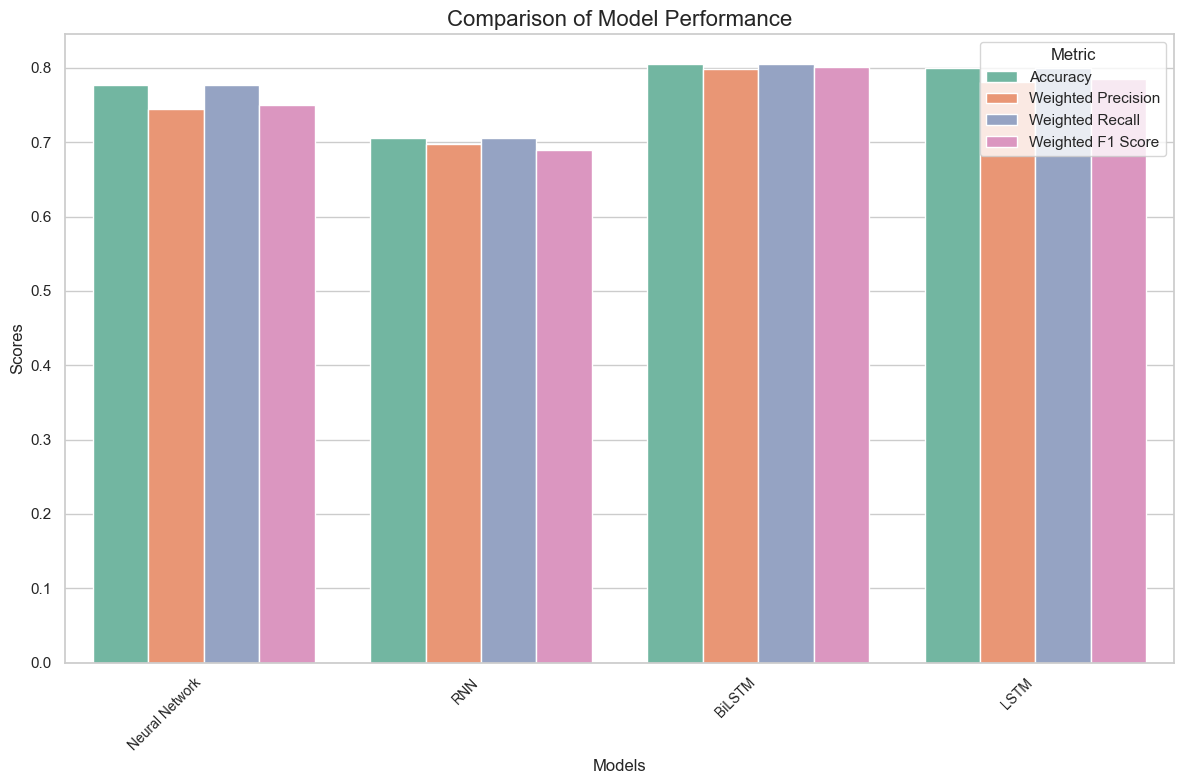
\includegraphics[width=\linewidth]{img/paper_2/Comparision Plot.png}
		\caption{Accuracy Comparison Across All Models}
		\label{fig:accuracy_comparison}
	\end{minipage}
	\hfill
	\begin{minipage}{0.48\textwidth}
		\centering
		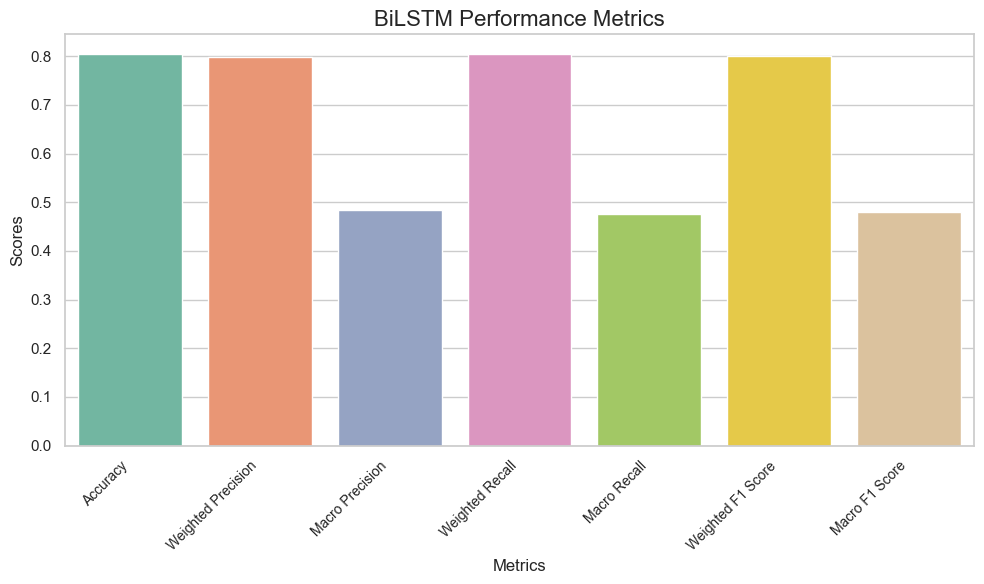
\includegraphics[width=\linewidth]{img/paper_2/BILSTM.png}
		\caption{Bi-LSTM Model Performance}
		\label{fig:bilstm_performance}
	\end{minipage}
	
	\vspace{0.5cm}
	
	\begin{minipage}{0.48\textwidth}
		\centering
		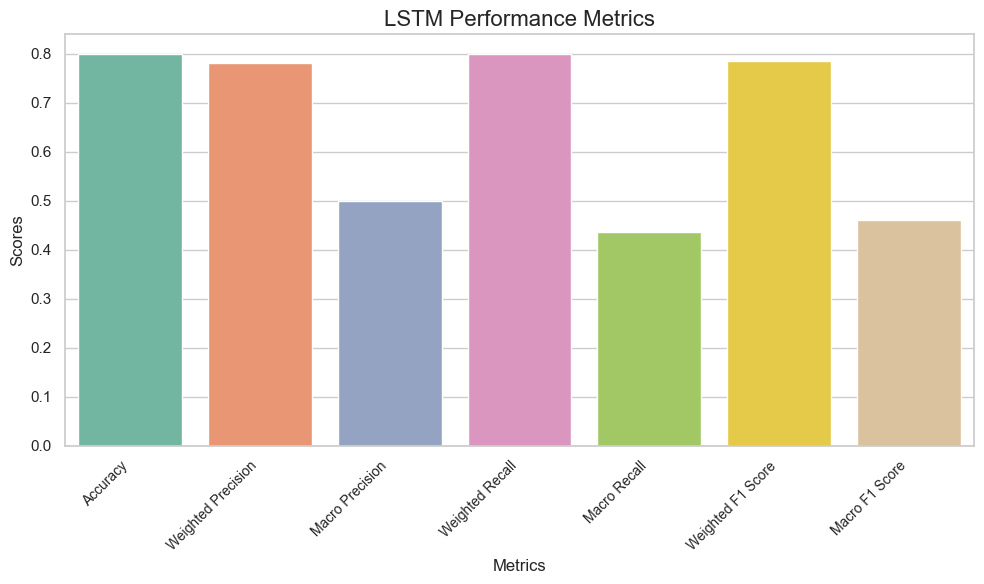
\includegraphics[width=\linewidth]{img/paper_2/LSTM.png}
		\caption{LSTM Model Performance}
		\label{fig:lstm_performance}
	\end{minipage}
	\hfill
	\begin{minipage}{0.48\textwidth}
		\centering
		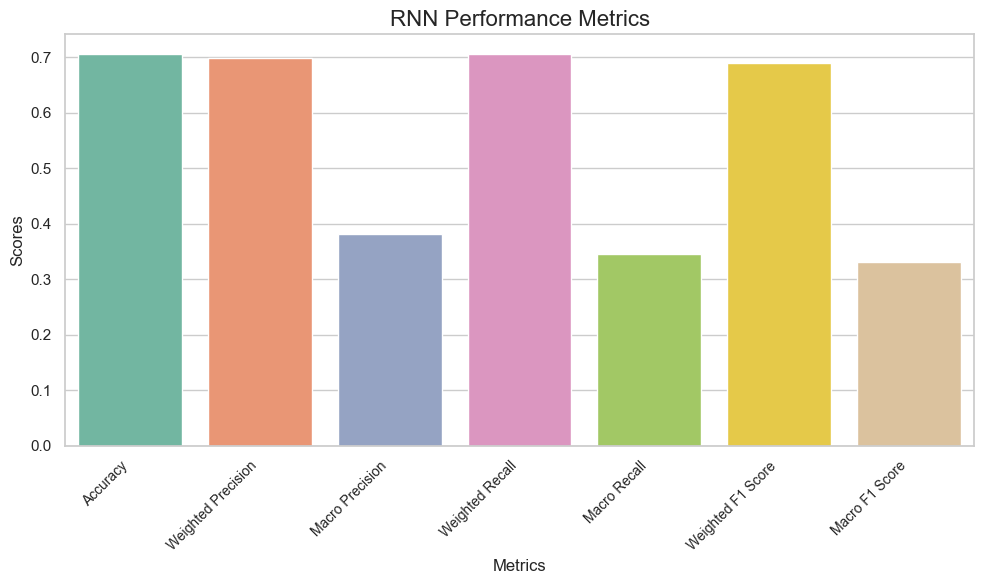
\includegraphics[width=\linewidth]{img/paper_2/RNN.png}
		\caption{RNN Model Performance}
		\label{fig:rnn_performance}
	\end{minipage}
\end{figure}

\begin{figure}[H]
	\centering
	\begin{minipage}{0.48\textwidth}
		\centering
		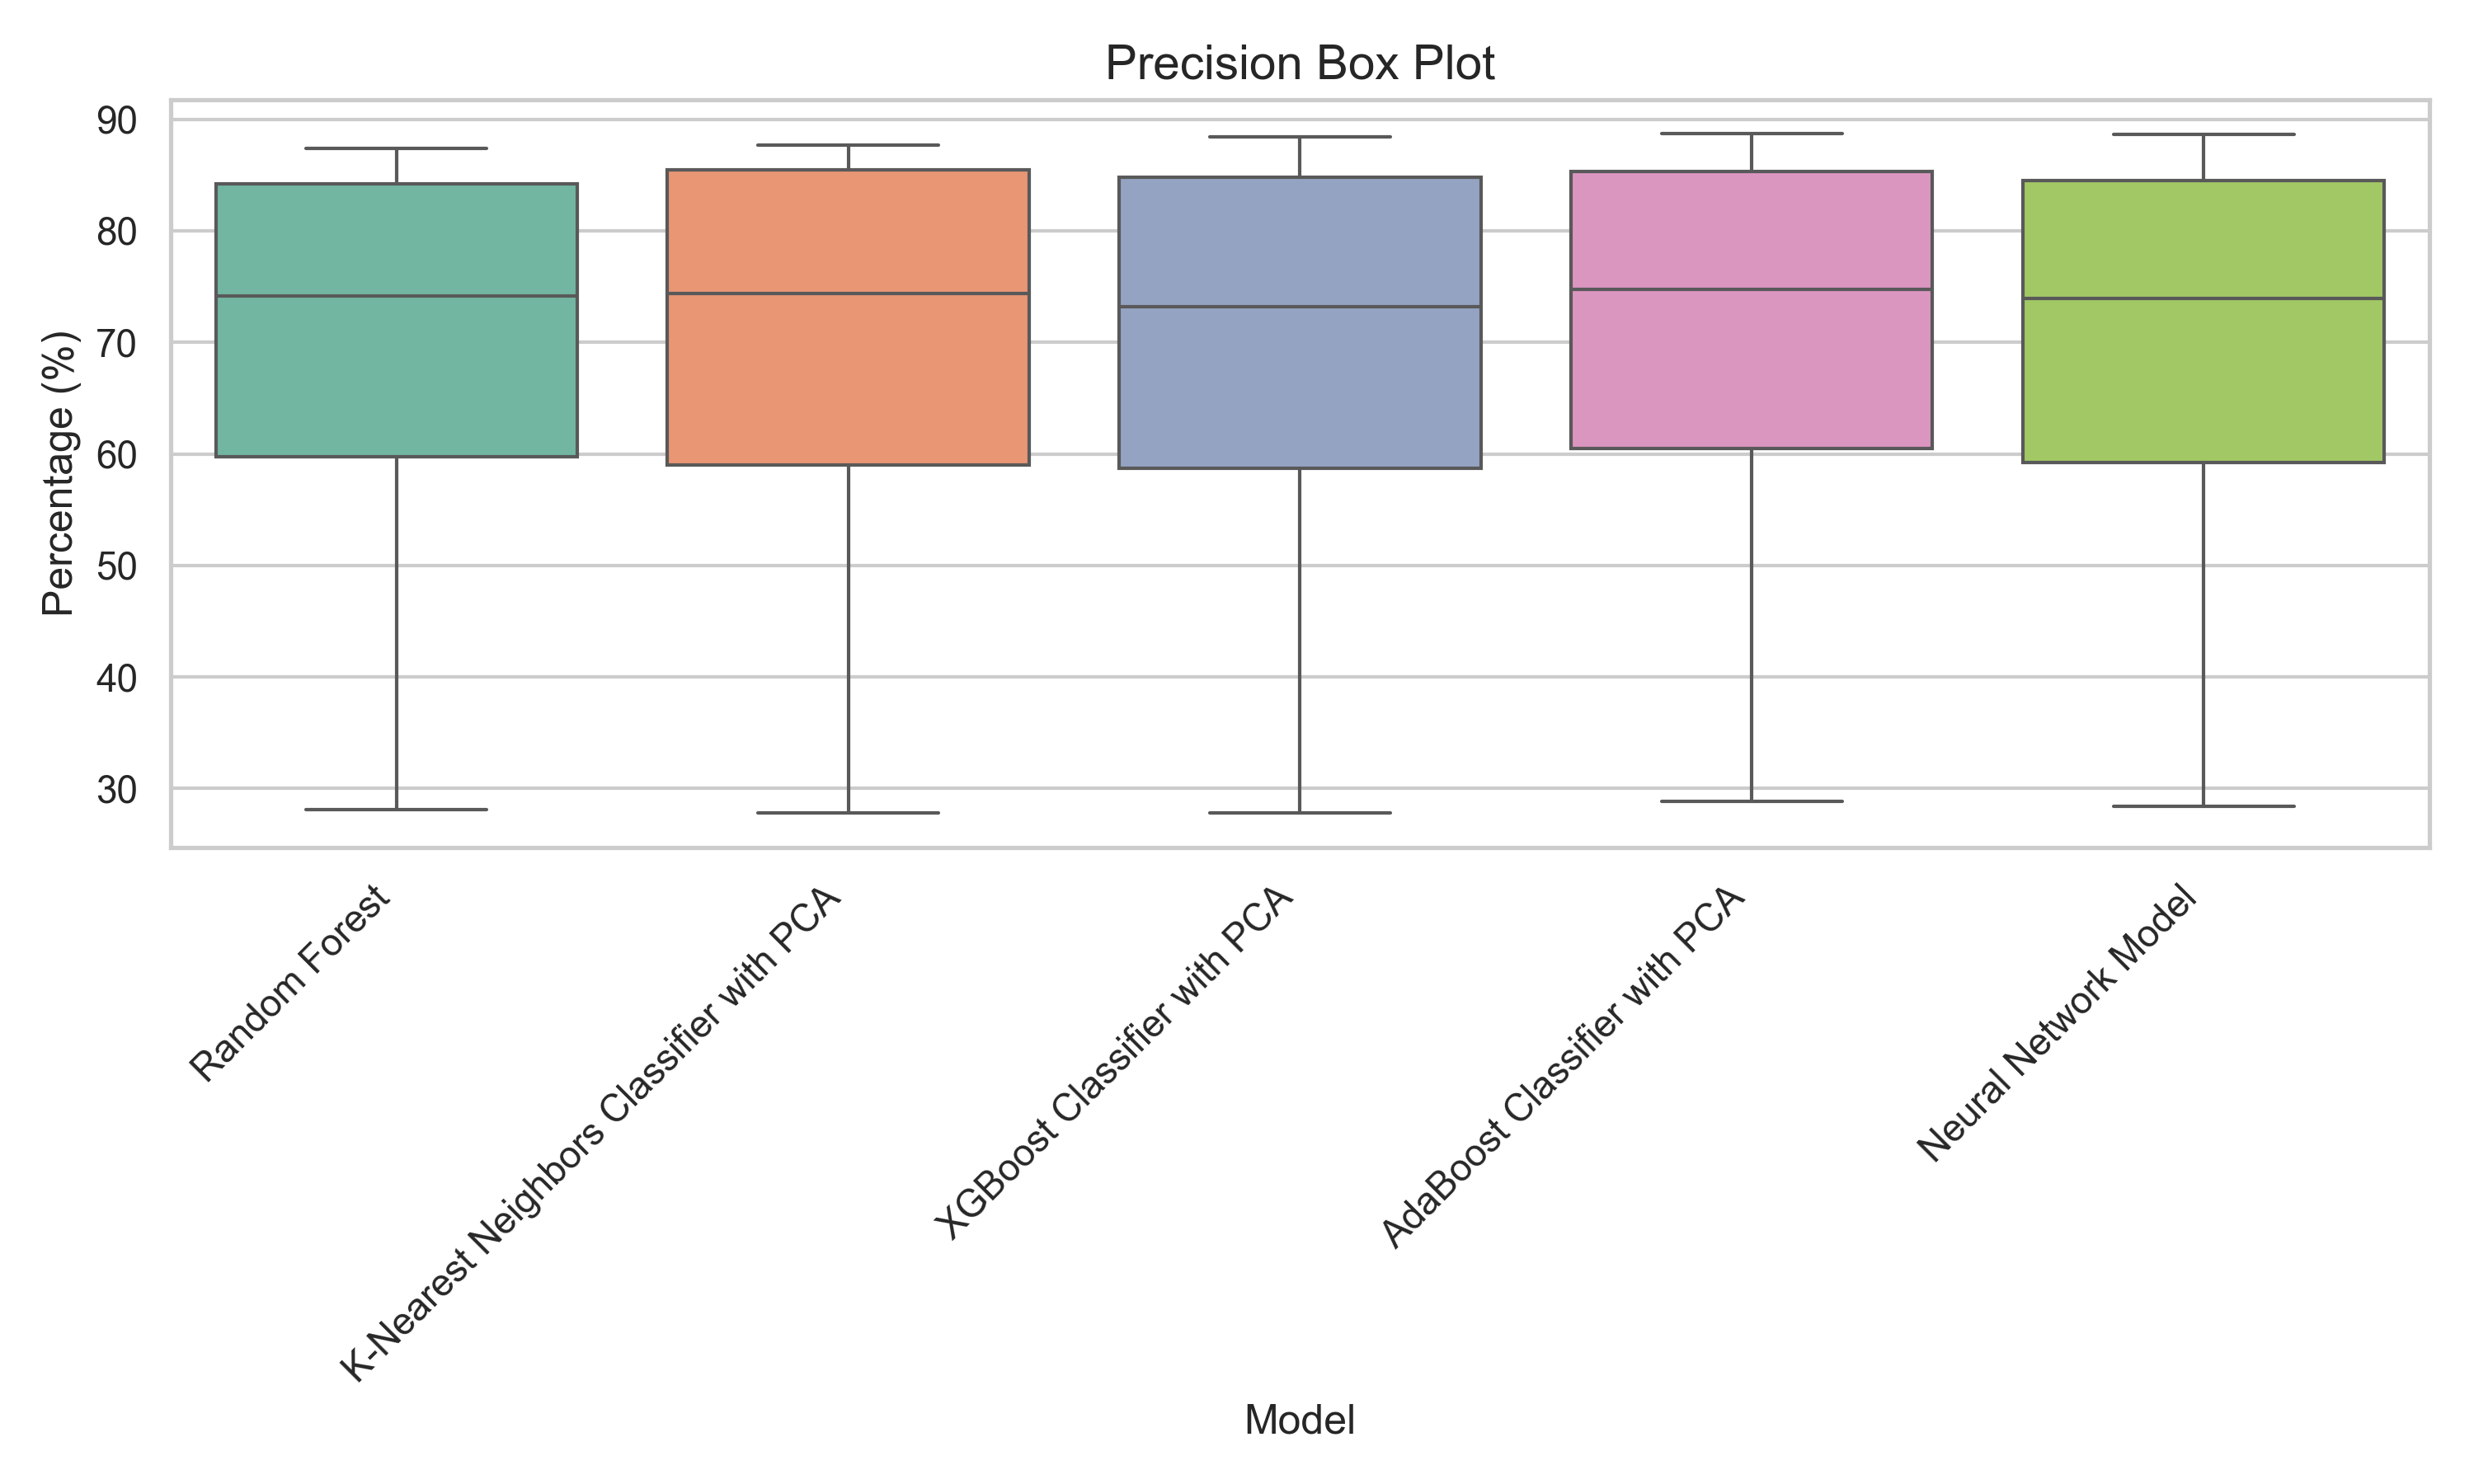
\includegraphics[width=\linewidth]{img/paper_2/Precision_box_plot}
		\caption{Box Plot of ML Precision Across Models}
		\label{fig:precisionboxplot}
	\end{minipage}
	\hfill
	\begin{minipage}{0.48\textwidth}
		\centering
		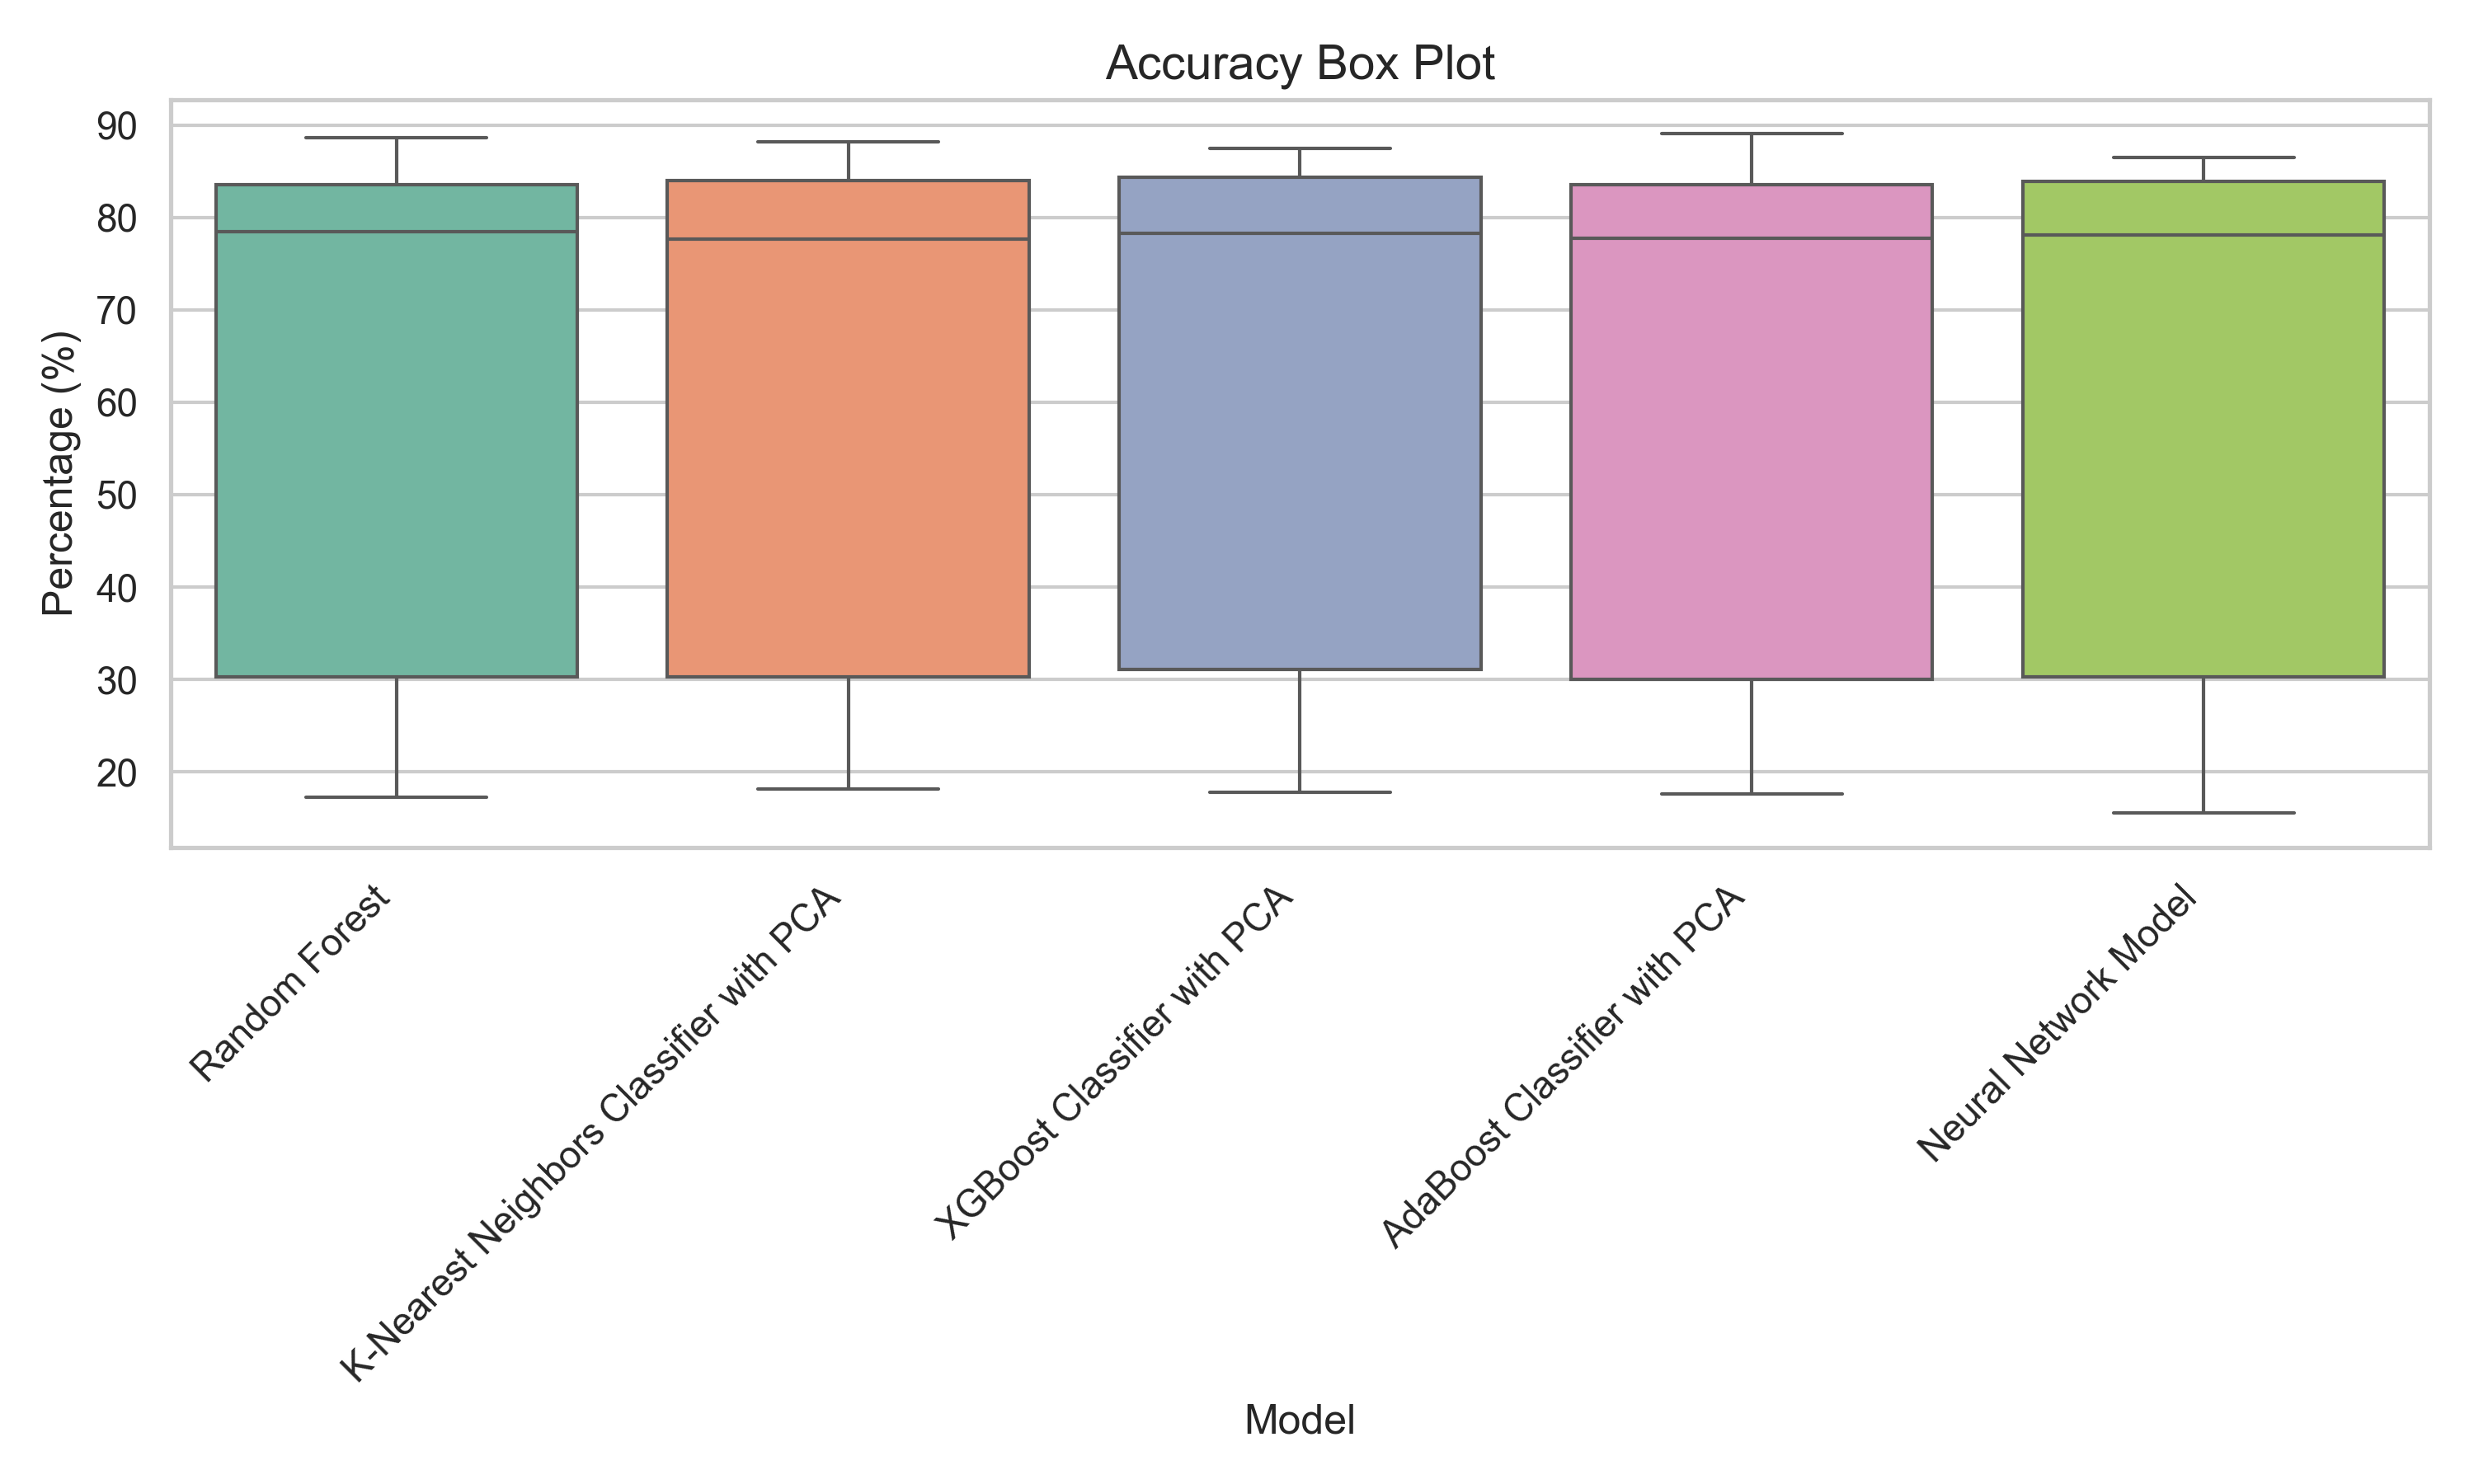
\includegraphics[width=\linewidth]{img/paper_2/Accuracy_box_plot}
		\caption{Box Plot of ML Accuracy Across Models}
		\label{fig:accuracyboxplot}
	\end{minipage}
\end{figure}
